%!TEX root = Thesis.tex

\chapter{Coordination Complexes with Platinum(II) and Palladium(II)}
\chaptermark{Platinum(II) and Palladium(II) Complexes}
\label{ch:platinumII}

Coordination complexes of palladium are used as catalysts for a wide range of reactions including cross-coupling, allylic alkylation and various carbonylation reactions, which are important on both laboratory and industrial scales.\cite{Dierkes1998, Freixa2003, Nicolaou2005, Peris2004, Shen2008, Suzuki1999, Wu2013, Simeone2010, Trost2012, Wagaw1999}  The high reactivity of palladium complexes can render them difficult to characterise and study.  Platinum and palladium have similar overall reactivity patterns.  However, platinum complexes are typically more inert than their corresponding palladium analogues to processes such as ligand exchange and redox changes.\cite{Chianese2007}.  The presence of a spin active isotope \Pt{} (34\% abundant) can result in coupling in the NMR spectra, which can give additional information about the nature of the complexes.  This makes platinum a useful model for the chemistry of palladium.  

Seven reports have been published investigating the catalytic activity of palladium complexes using \tBuxantphos{}.  These include the N-arylation and alkylation of amines, cross-coupling of thiols and aryl bromides or triflates, Suzuki cross-coupling, hydroesterificaton of methyl oleate, aminocarbonylation of hetero(aryl) bromides, and the methylation of alkynyl C-H bonds with dimethyl sulfonium ylides.\cite{Mispelaere2005, Cabello2007, Ashcroft2013, Behr2013, Friis2014, Dang2013, Liu2013c}  In the N-arylation of heterocyclic diamines the \tBuxantphos{} system showed little activity (\textless{} 1\%), whereas the \Phxantphos{} system was more successful (40\%).\cite{Cabello2007}   In the N-alkylation of aniline with benzyl alcohol the \tBuxantphos{} system gave 100\% conversion at 100\degC{} while the \Phxantphos{} reaction at 110\degC{} only gave 63\%.\cite{Dang2013}  The cross-coupling of butane thiol with phenyl triflates in xylene at 140\degC{} produced only trace amounts of the product using \tBuxantphos{} while an 80\% yield was obtained with \Phxantphos{}.\cite{Mispelaere2005}  The \Phxantphos{} complex was also more reactive in the Suzuki cross-coupling of 2-(4-bromophenyl)-5-chloropyrazine with a benzimidazole boronic ester giving a 83\% yield compared to only 5\% with \tBuxantphos{}.\cite{Ashcroft2013}  The same lack of activity was observed for the hydroesterification of methyl oleate, with no conversion obtained for \tBuxantphos{} compared to 70\% for \Phxantphos{}.  In the methylation of alkynyl C-H bonds with dimethyl sulfonium ylides, the \tBuxantphos{} ligand produced a greater yield than the \Phxantphos{} ligand (46\% compared to 15\%).\cite{Liu2013c}  Together, these studies suggest differences in the coordination chemistry and reactivity of the \tBuxantphos{} and \Phxantphos{} ligands.  However, little research into the coordination chemistry of \tBuxantphos{} has been performed.  

Only two palladium complexes of \tBuxantphos{} have been reported.  The X-ray crystal structure of [Pd(\tBuxantphos\ce{)Cl2}] was reported to the \gls{CSD} in 2011 (CSD-XARXAR),\cite{Allen2002} however a research paper including synthetic details has not been published.  The crystal structure (Figure \ref{PdtBuxantphos}) has three molecules in the asymmetric unit each showing a distorted \trans{} geometry with P-Pd-P angles of 160.59(4), 161.97(3) and 161.31(4)\degrees{}.  These are larger than the 100.61(5) and 100.92(7)\degrees{} for [Pd(\Phxantphos)\ce{Cl2}] with different solvates.\cite{Allen2002, Johns2006, Jahromi2012}  The difference in the bite-angles and geometries of the complexes that form may explain the difference in the catalytic reactivity of the complexes.  The other complex reported for \tBuxantphos{} showed an unusual monodentate coordination mode (Figure \ref{Pdmetallacycle}).\cite{Friis2014}  This is not a common coordination mode for the xantphos ligands and the same complex was also formed with \Phxantphos{}.  In an aminocarbonylation reaction the \Phxantphos{} complex gave a 92\% isolated yield, while no product was observed using the \tBuxantphos{} system.  The reason for this difference was not addressed in the publication.

\begin{figure}[htbp]
\begin{center}
\vspace{0.5cm}
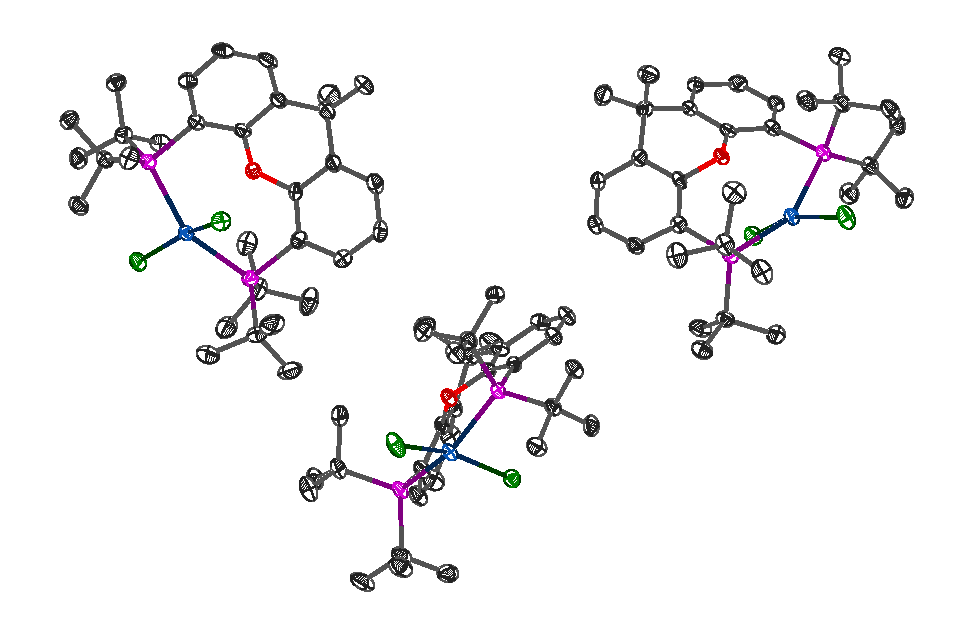
\includegraphics[width=\textwidth]{../Othercrystals/PdtBuxantphos.eps}
\caption[X-ray crystal structure of [Pd(\tBuxantphos)\ce{Cl2}{]}]{X-ray crystal structure of [Pd(\tBuxantphos)\ce{Cl2}] (CSD-XARXAR).\cite{Allen2002}  Hydrogen atoms and solvent of crystallisation omitted for clarity.}
\vspace{0.2cm}
\label{PdtBuxantphos}
\end{center}
\end{figure}

\begin{figure}[htbp]
\begin{center}
\vspace{0.5cm}
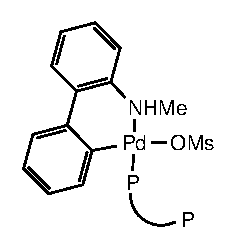
\includegraphics{../Figures/Pdmetallacycle.eps}
\caption[Previously reported palladium complex of \tBuxantphos{} and \Phxantphos{}]{Previously reported palladium complex with PP = \tBuxantphos{} or \Phxantphos{}.\cite{Friis2014}}
\vspace{0.2cm}
\label{Pdmetallacycle}
\end{center}
\end{figure}

Metal halide complexes are ubiquitous in coordination chemistry.  They form a number of complexes that are active catalysts, and are widely used as starting points for the synthesis of more complex systems.  Platinum halide complexes are also of interest due to their potential as chemotherapeutics.  Complexes such as, \cis{}-platin \ce{[PtCl2(NH3)2]} and its derivatives are now an important part of  several treatment protocols and have improved the prognosis for many cancer patients, for example, the cure rate of testicular cancer has increased from less than 10\%{} to over 90\%.\cite{Wilson2013}

The coordination chemistry of \Phxantphos{} on palladium has been the subject of a number of studies,\cite{Zuideveld2002, Raebiger2004, Bakhmutov2012, Miedaner2004, Klingensmith2006, Petocz2004, Yin2002}  though few have investigated the coordination chemistry with platinum. Catalytic systems frequently involve palladium in both the 0 and +2 oxidation states, hence it is important that both are studied.\cite{Tsuji1995}  Investigation into the coordination chemistry of the \tBuxantphos{} ligands with platinum and palladium(0) was reported in Chapter \ref{ch:platinum0}.  This chapter will present work on the coordination chemistry of the three \tBuxantphos{} ligands with platinum and palladium(II) in order to investigate the differences and similarities in the chemistry of the \tBuxantphos{} ligands with the \Phxantphos{} ligands.  

%======================================================================
%Copied from platinum0 section

%Previous work with wide bite-angle ligands based on xanthene backbones has encountered difficulties when attempting coordination to Pt and Pd(II).  The reactions proceed giving either a mixture of products\cite{Malaise2006, Veen2000b} or dynamic processes \cite{Veen2000b}.  The square planar geometries preferred by these metals in their +2 oxidation states, allows for either \cis{} or \trans{} coordination of diphosphines with ideal bite-angles close to 90 or 180\degrees{}.  The xanthene based ligands have bite-angles of generally around 120\degrees{} and limited flexibility.  Hence often both \cis{} and \trans{} complexes form or an interconversion between the two is observed.  As such more work has been carried out with metals that are less rigid in their coordination geometries, such as Rh.  

%Platinum xantphos complexes have shown particular activity in the allylation of amines.\cite{Mora2008}

%Petocz2004 for information on cis and trans platinum xantphos complexes


%The coordination chemistry of the \tBuxantphos{} ligands with platinum(0) produced a number of platinum(II) complexes upon reaction (Chapter \ref{chapter:platinum0}).  This chapter presents research into the coordination chemistry of the three \tBuxantphos{} ligands with platinum(II) and palladium(II) precursors.

%======================================================================

\section[Reactions with Platinum Dichloride Starting Materials]{Reactions with Platinum Dichloride Starting \\Materials}

The reactivity of the \tBuxantphos{} ligands towards platinum dichloride starting materials was initially investigated by studying the reaction of \tButhixantphos{} with a range of different starting materials in both \cis{} and \trans{} geometries: [Pt\ce{Cl2}(\acrshort{hex})], (\acrshort{hex} = \acrlong{hex}) \cis-[Pt\ce{Cl2(SEt2)2}], \cis-[Pt\ce{Cl2(MeCN)2}], \trans-[Pt\ce{Cl2(MeCN)}], and \trans-[Pt\ce{Cl2(^{t}BuCN)2}].  In a number of cases, the reaction was very slow and protonation of the \tButhixantphos{} ligand occurred faster than the formation of a platinum complex.  If a platinum complex was produced, it was the same species irrespective of the starting material or conditions of the reaction.  The most successful result went to completion after 72 hours in toluene at 50\degC{} using [Pt\ce{Cl2}(\acrshort{hex})], which contains a readily displaced diene ligand.  In \ce{C6D6} the product appears in the \phosphorus{} NMR spectrum as a singlet at 32.9 ppm with a \JPtP{} value of 2700 Hz.  The value of the one-bond phosphorus-platinum coupling constant can give important information regarding the geometry of the complex.  In particular, the value of \JPtP{} is highly dependent on the \trans{}-influence of the ligand \trans{} to the phosphorus atom.\cite{Pregosin2012}  A value of 2700Hz for \JPtP{} is characteristic of mutually \trans{} phosphorus atoms, rather than phosphorus \trans{} to a chloride (\JPtP{} = 3200--3800 Hz).\cite{Rigamonti2010, Appleton1978, Pregosin1980}  Hence, the product of the reaction between \tButhixantphos{} and [Pt\ce{Cl2}(\acrshort{hex})] is \trans{}-[Pt(\tButhixantphos)\ce{Cl2}] (Scheme \ref{scheme:platinumdichloride}).

\begin{scheme}[ht]
\begin{center}
\vspace{0.5cm}
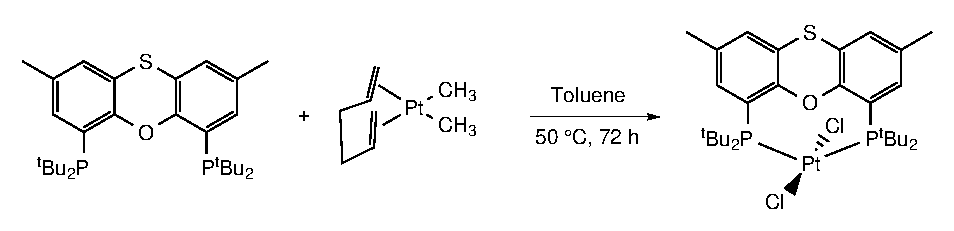
\includegraphics{../Schemes/Platinumdichloride.eps}
\caption[Synthesis of [Pt(\tButhixantphos)\ce{Cl2}{]}]{Synthesis of [Pt(\tButhixantphos)\ce{Cl2}].  \emph{Reagents and conditions:} (i) toluene, 50\degC, 3 days.}
\vspace{0.2cm}
\label{scheme:platinumdichloride}
\end{center}
\end{scheme}
\vspace{0.2cm}

[Pt(\tButhixantphos)\ce{Cl2}] is dark red in both \ce{C6D6} solution and the solid state.  This is unusual as platinum dichloride complexes are typically pale, or yellow in colour.  Indeed the previously reported [Pt(\Phxantphos)\ce{Cl2}] complex is a white solid.\cite{Ohshima2009}  This suggests that [Pt(\tButhixantphos)\ce{Cl2}] is unusual from an electronic perspective, which may be the result of a strained coordination geometry.  

Dark red crystals of [Pt(\tButhixantphos)\ce{Cl2}] suitable for X-ray diffraction were grown by inwards diffusion of diethyl ether into a dichloromethane solution of the complex.  The structure is shown in Figure \ref{crystalthixantphosplatinumdichloride}, with a side-on view in Figure \ref{crystalthixantphosplatinumdichlorideside}.  The complex crystallises in the monoclinic crystal system in the space group P2\sub{1}/c.  Selected bond lengths and angles are given in Table \ref{table:crystalthixantphosplatinumdichloride:lengths}, and the crystallographic data is given in Table \ref{table:crystalthixantphosplatinumdichloride:data}.  

\begin{figure}[htbp]
\begin{center}
\vspace{0.5cm}
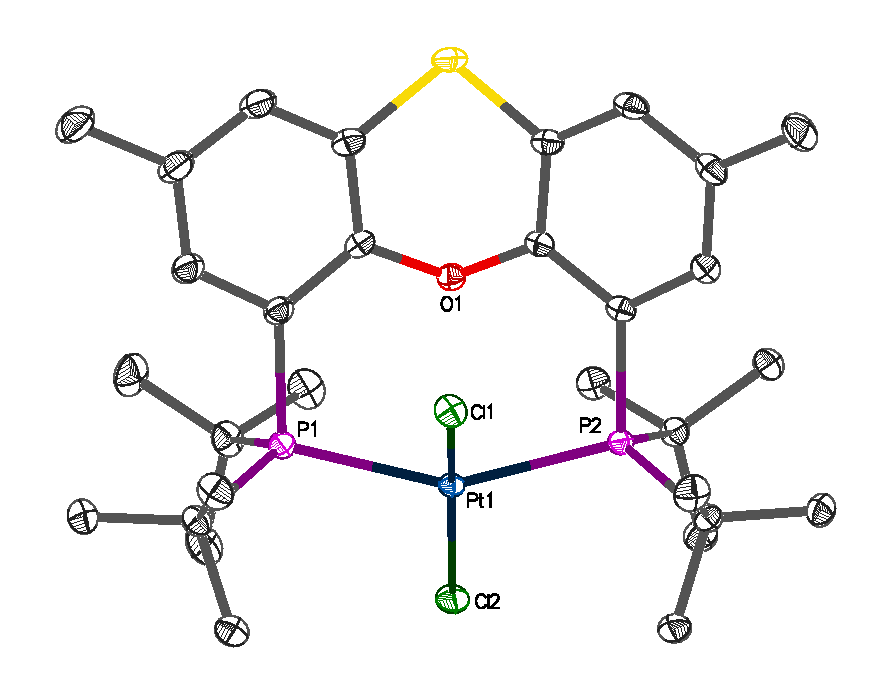
\includegraphics[scale=0.8]{../Figures/Crystalthixantphosplatinumdichloride.eps}
\caption[X-ray crystal structure of [Pt(\tButhixantphos)\ce{Cl2]}]{X-ray crystal structure of [Pt(\tButhixantphos)\ce{Cl2]} (50\% probability thermal ellipsoids). Hydrogen atoms omitted for clarity.}
\label{crystalthixantphosplatinumdichloride}
\end{center}
\end{figure}
\vspace{0.2cm}

\begin{figure}[htbp]
\begin{center}
\vspace{0.5cm}
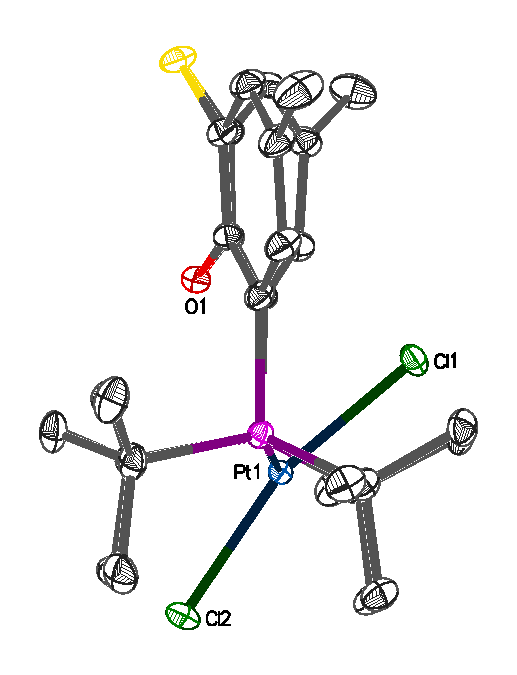
\includegraphics[scale=0.8]{../Figures/Crystalthixantphosplatinumdichlorideside.eps}
\caption[X-ray crystal structure of [Pt(\tButhixantphos)\ce{Cl2]}, side view]{X-ray crystal structure of [Pt(\tButhixantphos)\ce{Cl2]}, side view (50\% probability thermal ellipsoids). Hydrogen atoms omitted for clarity.}
\label{crystalthixantphosplatinumdichlorideside}
\end{center}
\end{figure}
\vspace{0.2cm}

\begin{table}[ht]
\caption[Bond distances (\AA) and angles (\degrees) of [Pt(\tButhixantphos)\ce{Cl2]}]{Selected bond distances (\AA) and angles (\degrees) of [Pt(\tButhixantphos)\ce{Cl2]}.}
\label{table:crystalthixantphosplatinumdichloride:lengths}
\small
\begin{center}
\begin{tabular}{l l l l}
	\toprule
	\multicolumn{2}{l}{\bfseries{~Bond distances (\si{\angstrom})}} & \multicolumn{2}{c}{\bfseries{Bond angles (\degrees)}} \\
	\midrule		
	~P1...P2		~~&~~4.5037(6)~~	&~~P1-Pt-P2			&~~151.722(15)~~	\\	
	~P1-Pt		~~&~~2.3205(4)~~	&~~Cl1-Pt-Cl2			&~~164.235(15)~~	\\
	~P2-Pt		~~&~~2.3239(4)~~	&~~P1-Pt-Cl1			&~~87.11(15)~~	\\
	~Pt-Cl1		~~&~~2.3209(4)~~	&~~P1-Pt-Cl2			&~~95.939(16)~~	\\
	~Pt-Cl2		~~&~~2.3098(4)~~	&~~P2-Pt-Cl1			&~~86.699(14)~~	\\
	~Pt...O		~~&~~2.8016(11)~~	&~~P2-Pt-Cl2			&~~96.917(15)~~	\\
	~				&			&~~Ring 1-Ring 2		&~~139.11(6)~~	\\
	\bottomrule{}
\end{tabular}
\end{center}
\end{table}

\begin{table}[htp]
\small
\caption[Crystallographic data and structure refinement of [Pt(\tButhixantphos)\ce{Cl2]}]{Crystallographic data and structure refinement of [Pt(\tButhixantphos)\ce{Cl2]}.} 
\label{table:crystalthixantphosplatinumdichloride:data}
\small
\begin{center}
\begin{tabular}{l l}
	\toprule
	\bfseries{Empirical formula}~~& \bfseries{\ce{C30H46Cl2OP2PtS}}\\
	\midrule
	Formula weight	 							& 782.66\\
	Temperature/K	 							& 284.87(10)\\
	Crystal system	 							& monoclinic\\
	Space group	 							& P2\sub{1}/c\\
	a$/$\si{\angstrom}							& 15.26769(8)\\
	b$/$\si{\angstrom} 							& 10.98650(7)\\
	c$/$\si{\angstrom}							& 19.05134(13)\\
	$\alpha/$\degrees							& 90\\
	$\beta/$\degrees							& 95.2318(5)\\
	$\gamma/$\degrees							& 90\\
	Volume$/$\si{\angstrom\cubed}  				& 3182.33(3)\\
	Z	 									& 4\\
$\rho$\sub{calc} \si{\milli\gram}$/$\si{\milli\metre\cubed} 	& 1.634\\
\si{\micro}$/$\si{\milli\metre} 						& 4.766\\
F(000)	 									& 1568.0\\
Crystal size$/$\si{\milli\metre}	 					& 0.27 x 0.14 x 0.08\\
Radiation	 									& MoK$\alpha$ ($\lambda$ = 0.71073)\\
2$\theta$ range for data collection					& 5.264 to 75.522\degrees\\
Index ranges	 								& -25 $\leq$ h $\leq$ 25, -15 $\leq$ k $\leq$ 18, -32 $\leq$ l $\leq$ 31\\
Reflections collected	 							& 49341\\
Independent reflections	 						& 16242 [R\sub{int} = 0.0277, R\sub{sigma} = 0.0333]\\
Data$/$restraints$/$parameters					& 16242$/$0$/$348\\
Goodness-of-fit on F$^{2}$	 					& 1.076\\
Final R indexes [I$>$=2$\sigma$ (I)]	 				& R\sub{1} = 0.0240, wR\sub{2} = 0.0445\\
Final R indexes [all data]	 						& R\sub{1} = 0.0351, wR\sub{2} = 0.0486\\
Largest diff. peak/hole / e \si{\per\angstrom\cubed}		& 1.46/-1.27	\\
	\bottomrule
\end{tabular}
\end{center}
\end{table}

%The crystal structure of [Pt(\tButhixantphos)\ce{Cl2}] (Figure \ref{crystalthixantphosplatinumdichloride}) shows a distorted \trans-coordination, consistent with the NMR data.  The sum of the angles around the platinum is 366.665\degrees{}, indicating severe distortion from the ideal coordination plane. 

The crystal structure of [Pt(\tButhixantphos)\ce{Cl2}] (Figure \ref{crystalthixantphosplatinumdichloride}) is distorted from the square-planar geometry typically observed for Pt(II) complexes.  The $\tau_{5}$ parameter has been used for many years to describe the shapes of five-coordinate complexes.\cite{Addison1984}  In 2007 a related $\tau_{4}$ parameter was introduced to describe the distortion of four-coordinate copper complexes between the ideal tetrahedral and square planar geometries.\cite{Yang2007}  The parameter is defined in Equation \ref{tau4} where $\alpha$ and $\beta$ are the two largest L-M-L angles in the four-coordinate complex.  The value of $\tau_{4}$ vary between 0 for an ideal square-planar complex to 1 for a tetrahedral complex.  Using the two largest angles for [Pt(\tButhixantphos)\ce{Cl2}] (P1-Pt-P2 = 151.722 and Cl1-Pt-Cl2 = 164.235) gives a value for $\tau_{4}$ of 0.31.  This indicates severe distortion from the expected square-planar geometry with the structure closest to a seesaw geometry.

\begin{equation}
\tau_{4} = \frac{360 -(\alpha+\beta)}{141}
\label{tau4}
\end{equation}
\vspace{0.1cm}

\begin{sloppypar}
The bite-angle of the \tButhixantphos{} ligand is 151.722(15)\degrees{} in [Pt(\tButhixantphos)\ce{Cl2}], which is significantly larger than the natural bite-angle determined by DFT (126.98\degrees{}, Section \ref{section:biteangle}).  This deviation is likely due to the influence of the platinum centre, which prefers a coordination geometry close to square-planar.  The bite-angle is unusual for complexes of the type [Pt(PP)\ce{Cl2}], where PP is either two monophosphine ligands or one diphosphine ligand. A search of the \gls{CSD} showed that the P-Pt-P angles of these complexes are very bi-modal, showing clear preference for the \cis{} 90\degrees{} or the \trans{} 180\degrees{} (Figure \ref{PtCl2graph}).\cite{Allen2002} The \tButhixantphos{} angle (151.722(15)\degrees) is situated between these two regions, with the closest \emph{bis}-monophosphine complex at 167.261, and the closest chelating diphosphine at 171.9(4)\degrees{}. Seven other \trans{}-dichloridoplatinum complexes which have chelating diphosphines have been reported (Figure \ref{crystal:transspanning}).\cite{Bachechi1992, Engeldinger2003, Newman2012, Owens2008, Beuken1997, Freixa2003b, Ruhland2007}  All of these have larger P-Pt-P angles than the \tButhixantphos{} complex (171.9(4)--180.00(0)\degrees{}).  The chelate ring size for these molecules (Figure \ref{crystal:transspanning}) ranges from 10--14 atoms, with the cyclodextrin-derived system having a ring size of 21 atoms (Figure \ref{OJUBAW}).  In contrast, the \tButhixantphos{} chelate ring contains only 8 atoms.  This relatively small chelation ring size, combined with the rigidity of the backbone is likely the reason for the distortion around the platinum centre as the \trans{} chelation puts strain on the \tButhixantphos{} ligand.  
\end{sloppypar}

\begin{figure}[htb]
\begin{center}
\vspace{0.5cm}
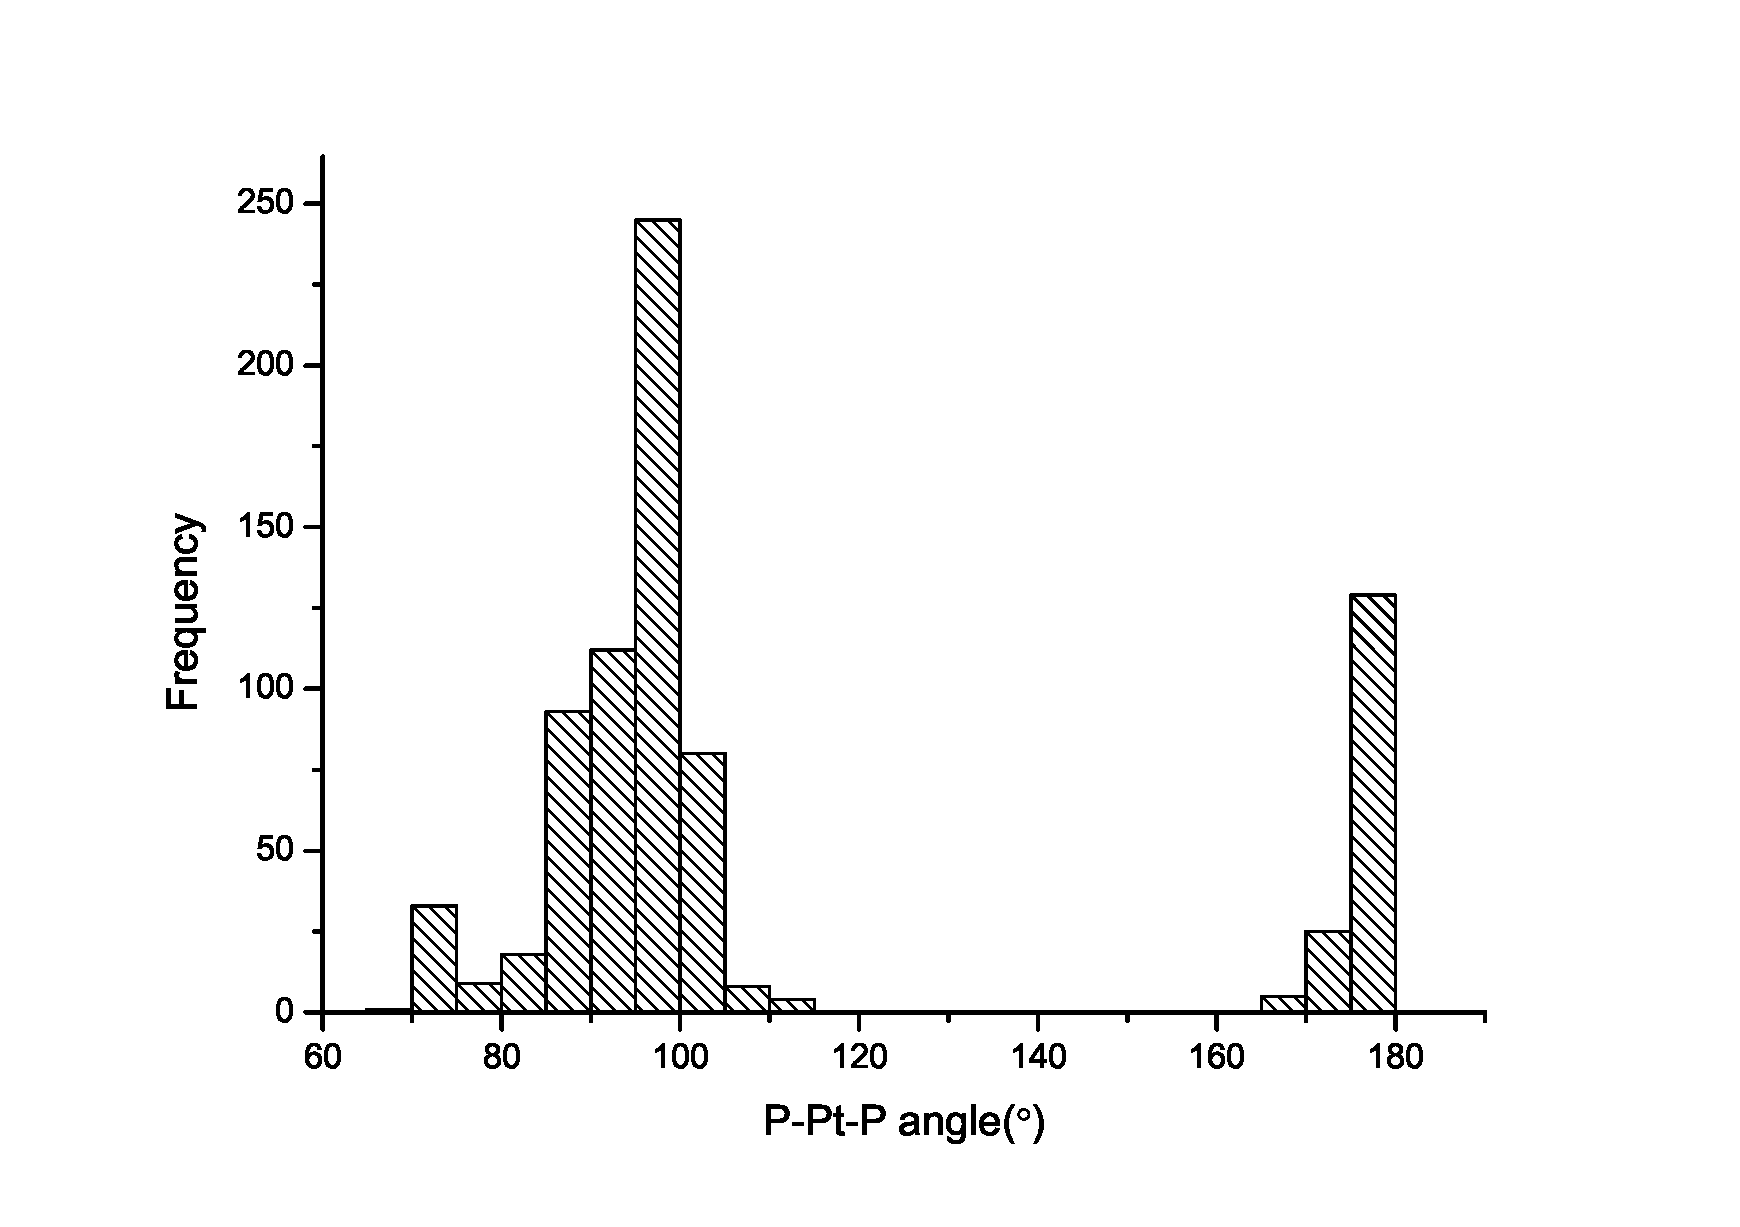
\includegraphics[width=\textwidth]{../Figures/Platinumdichloridegraph.eps}
\caption[Distribution of the P-Pt-P angles in \ce{[PtCl2(P2){]}} complexes]{Distribution of the P-Pt-P angles in crystal structures of \ce{[PtCl2(P2)]} where P = tertiary phosphine ligand, \ce{P2} = chelating diphosphine ligand.}
\vspace{0.2cm}
\label{PtCl2graph}
\end{center}
\end{figure}
\vspace{0.2cm}

\begin{figure}[htbp]
        \centering
        \begin{subfigure}[b]{0.4\textwidth}
                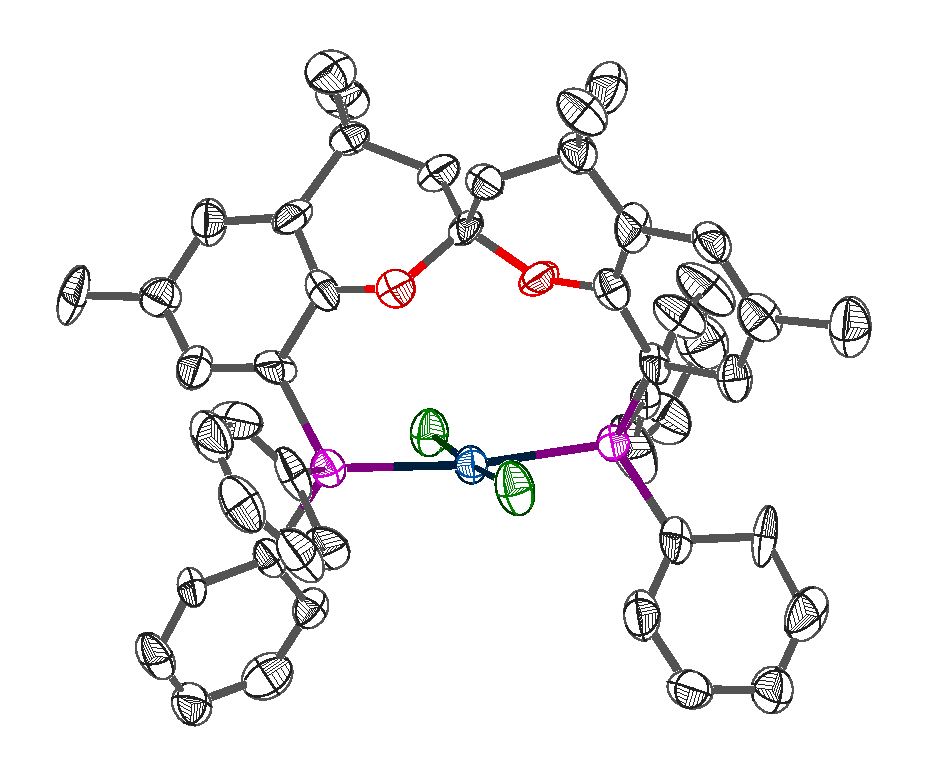
\includegraphics[width=\textwidth]{../Othercrystals/PtCl2/Trans/196130.eps}
                \caption{10 atoms, 171.9(4)\degrees{}\cite{Freixa2003b}}
                \label{WABXIH}
        \end{subfigure}%
        ~ 
        \begin{subfigure}[b]{0.3\textwidth}
                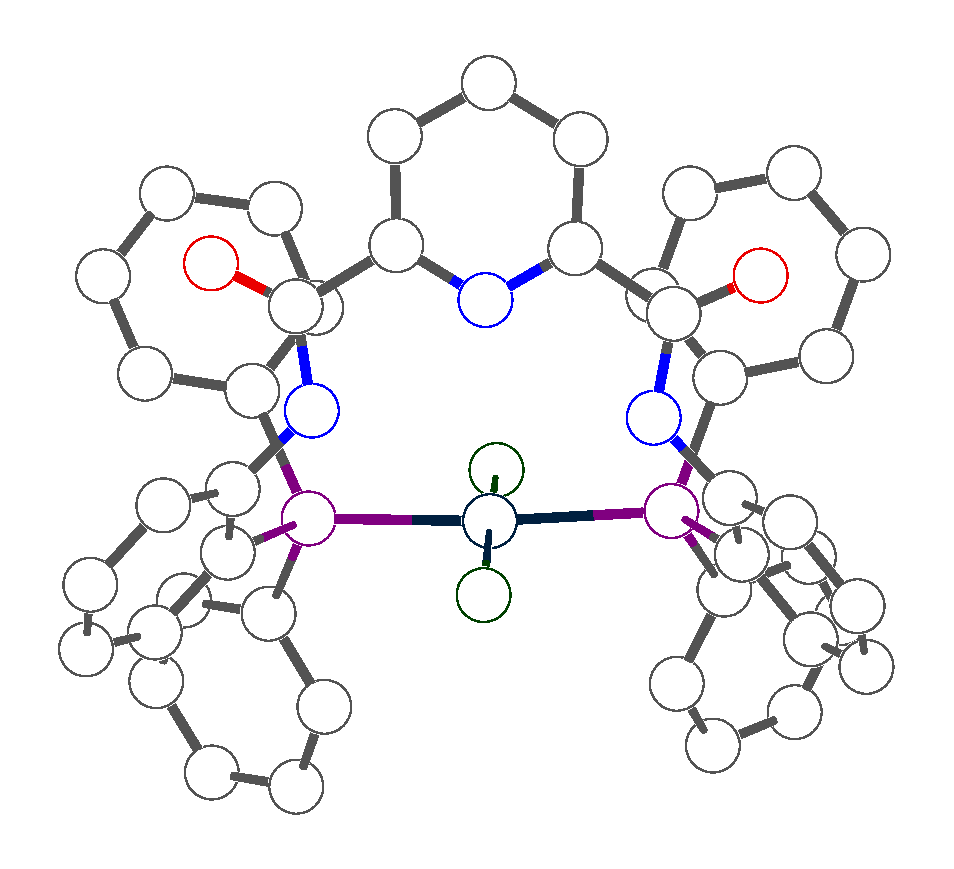
\includegraphics[width=\textwidth]{../Othercrystals/PtCl2/Trans/NURGAI.eps}
                \caption{14 atoms, 172.25(4)\degrees{}\cite{Beuken1997}}
                \label{NURGAI}
        \end{subfigure}
       \\
        \begin{subfigure}[b]{0.4\textwidth}
                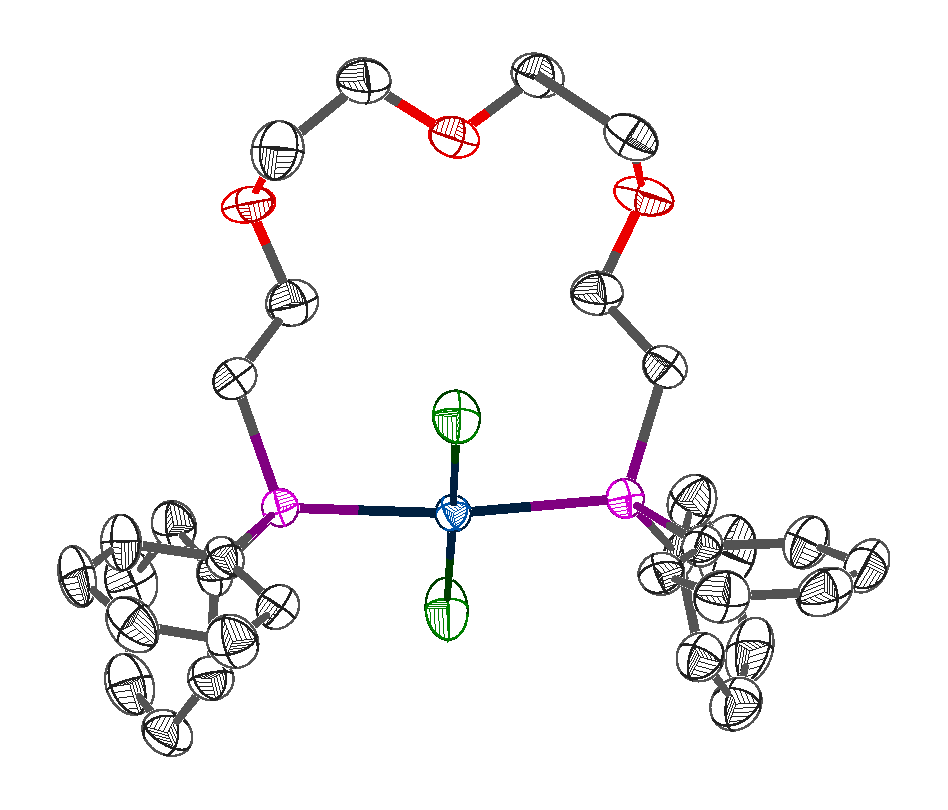
\includegraphics[width=\textwidth]{../Othercrystals/PtCl2/Trans/661699.eps}
                \caption{14 atoms, 173.01(6)\degrees{}\cite{Owens2008}}
                \label{HOJDUG}
        \end{subfigure}%
        ~
        \begin{subfigure}[b]{0.4\textwidth}
                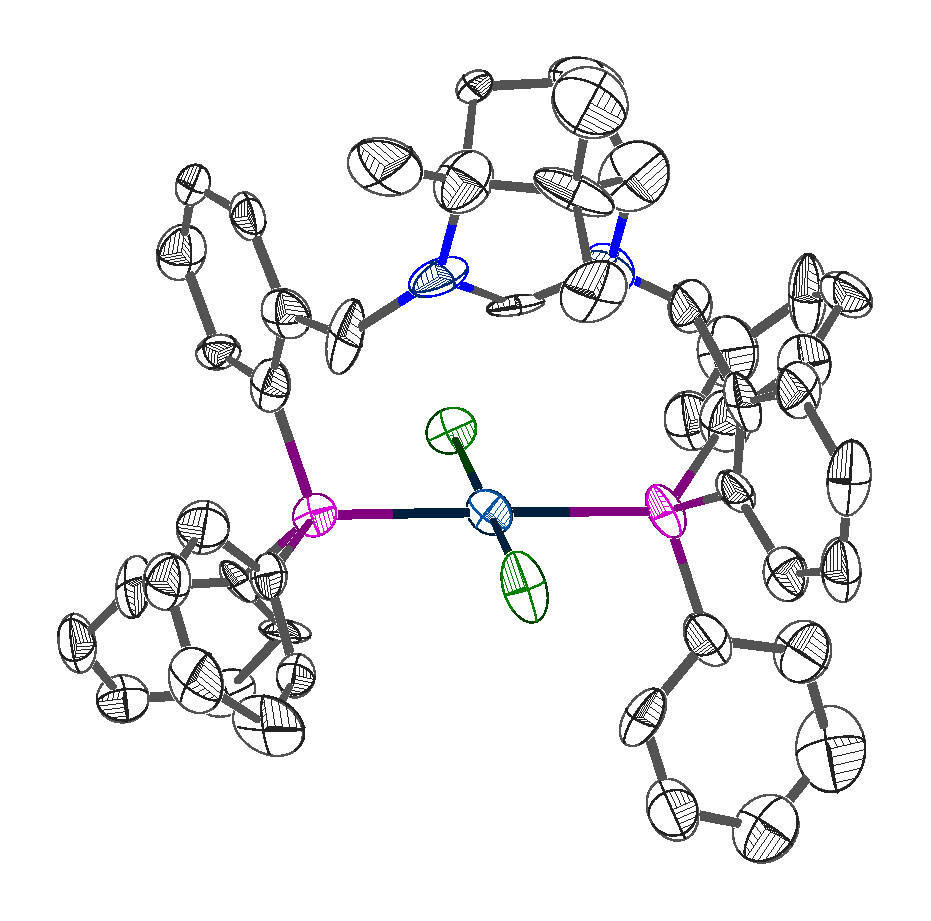
\includegraphics[width=0.8\textwidth]{../Othercrystals/PtCl2/Trans/891177.eps}
                \caption{12 atoms, 174.9(3)\degrees{}\cite{Newman2012}}
                \label{CAZXIM}
        \end{subfigure}
        \\
        \begin{subfigure}[b]{0.32\textwidth}
                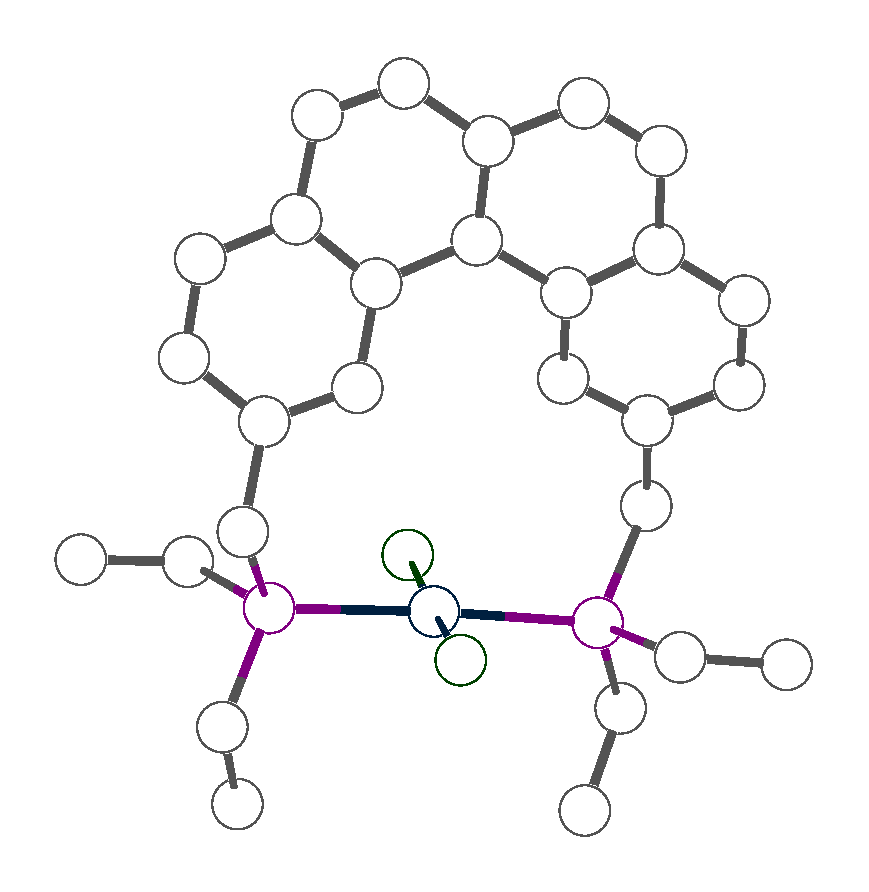
\includegraphics[width=\textwidth]{../Othercrystals/PtCl2/Trans/KOWHIN.eps}
                \caption{12 atoms, 177.1(3)\degrees{}\cite{Bachechi1992}}
                \label{KOWHIN}
        \end{subfigure}
        ~
        \begin{subfigure}[b]{0.32\textwidth}
                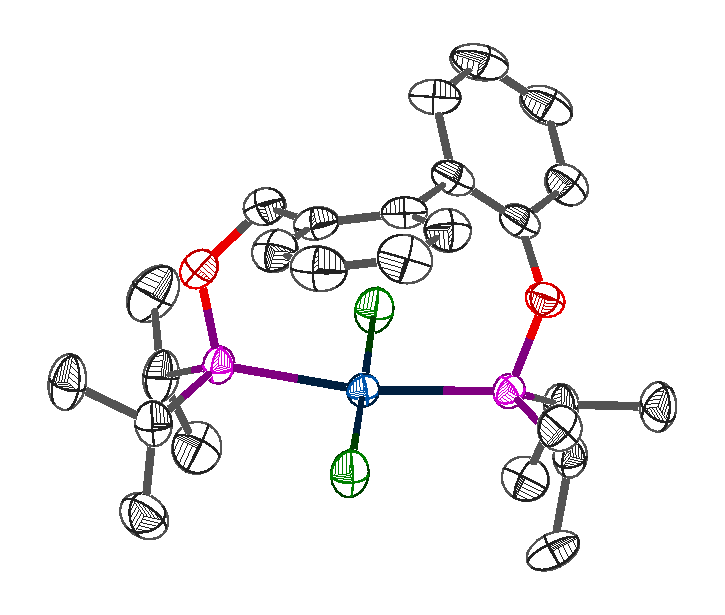
\includegraphics[width=\textwidth]{../Othercrystals/PtCl2//Trans/613904.eps}
                \caption{10 atoms, 177.77(6)\degrees{}\cite{Ruhland2007}}
                \label{WIBCIU}
        \end{subfigure}
        ~
        \begin{subfigure}[b]{0.32\textwidth}
                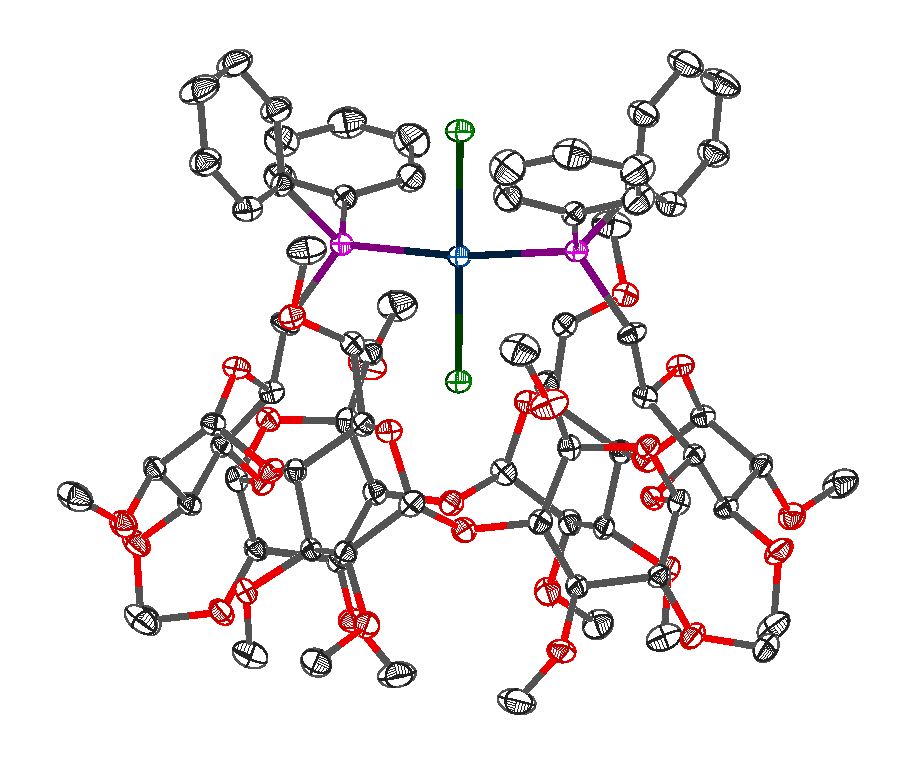
\includegraphics[width=\textwidth]{../Othercrystals/PtCl2/Trans/202109.eps}
                \caption{21 atoms, 180.00(0)\degrees{} \cite{Engeldinger2003}}
                \label{OJUBAW}
        \end{subfigure}
        \caption[X-ray crystal structures of dichloridoplatinum complexes with \trans-spanning diphosphine ligands]{X-ray crystal structures of dichloridoplatinum complexes with \trans-spanning diphosphine ligands.  The values given are the P-Pt-P angles.}
        \label{crystal:transspanning}
        \end{figure}
        
The P-Pt-P angle of [Pt(\tButhixantphos)\ce{Cl2}] (151.722(15)\degrees) is much larger than in the closest \cis{}-[Pt\ce{Cl2(P2)}] (\ce{P2} = chelating diphosphine) complexes (113.39(3))\degrees{} and 113.43(6)\degrees{}).  Both of these complexes contain xantphos ligands, indicating that the rigid xantphos backbone plays a role in forming species with larger bite-angles.\cite{Vlugt2003, Mora2008}  In addition to the two already mentioned, three other crystal structures for [Pt\ce{Cl2}(xantphos)] complexes have been reported (Figure \ref{crystal:otherPtCl2}).\cite{Duren2006, Duren2007, Niksch2010}  These complexes have crystallographically determined bite-angles of 99.17(3), 99.64(4) and 100.87(8)\degrees.  Although these are all \cis{} dichloride complexes it can be seen that the xantphos ligands have access to larger bite-angles than the ideal 90\degrees{} of the square-planar platinum(II) complexes.  In [Pt(\tButhixantphos)\ce{Cl2}] it is likely that the \trans{} coordination of the chloride ligands is the result of the increased steric demand of the \tBu{} substituents, which results in the larger observed bite-angle.  

\begin{figure}[htbp]
        \centering
        \begin{subfigure}[b]{0.45\textwidth}
                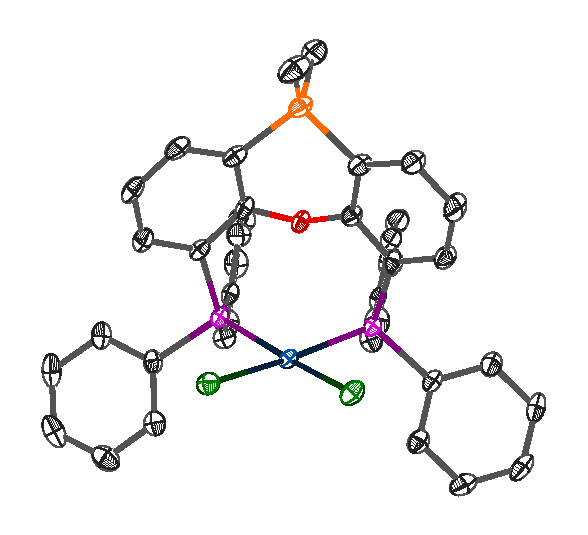
\includegraphics[width=\textwidth]{../Othercrystals/PtCl2/630063.eps}
                \caption{99.17(3)\degrees{}\cite{Duren2007}}
                \label{PtCl2SiPh}
        \end{subfigure}%
        ~ 
        \begin{subfigure}[b]{0.45\textwidth}
                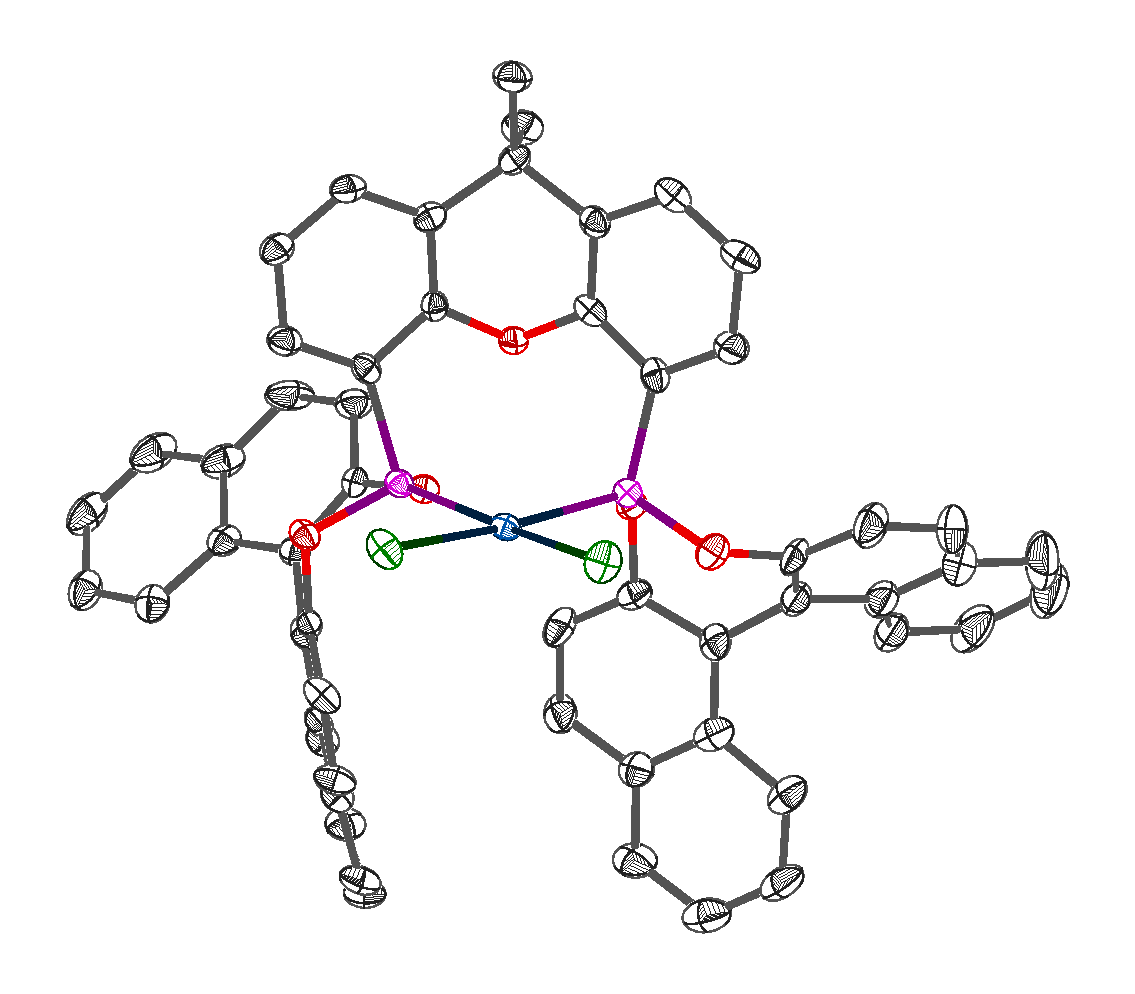
\includegraphics[width=\textwidth]{../Othercrystals/PtCl2/295949.eps}
                \caption{99.64(4)\degrees{}\cite{Duren2006}}
                \label{PtCl2BINAP}
        \end{subfigure}
        \\
        \begin{subfigure}[b]{0.45\textwidth}
                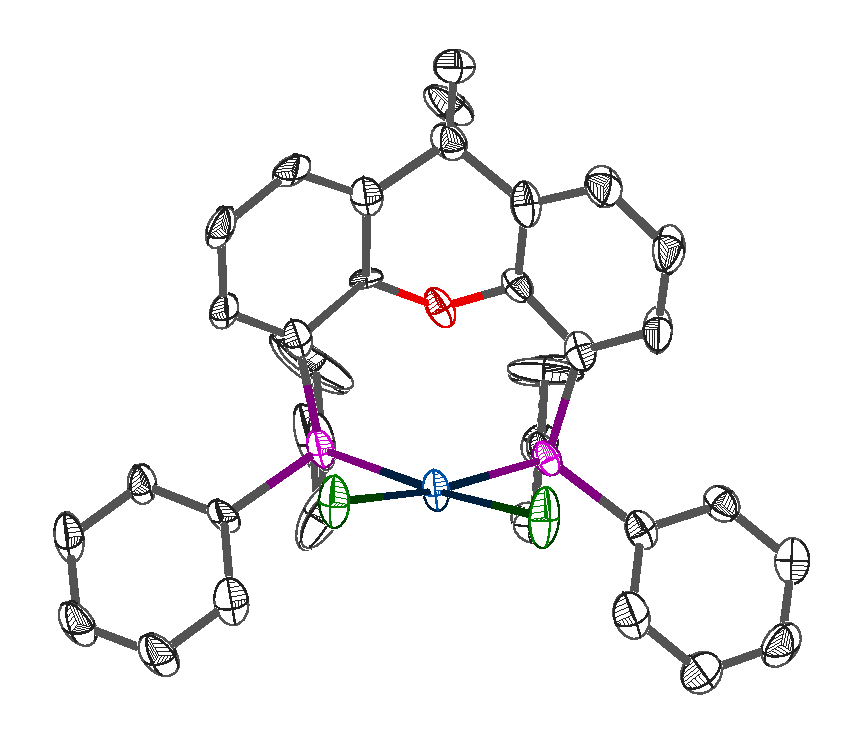
\includegraphics[width=\textwidth]{../Othercrystals/PtCl2/730506.eps}
                \caption{100.87(8)\degrees{}\cite{Niksch2010}}
                \label{PtCl2Cy}
        \end{subfigure}%
        ~ 
        \begin{subfigure}[b]{0.45\textwidth}
                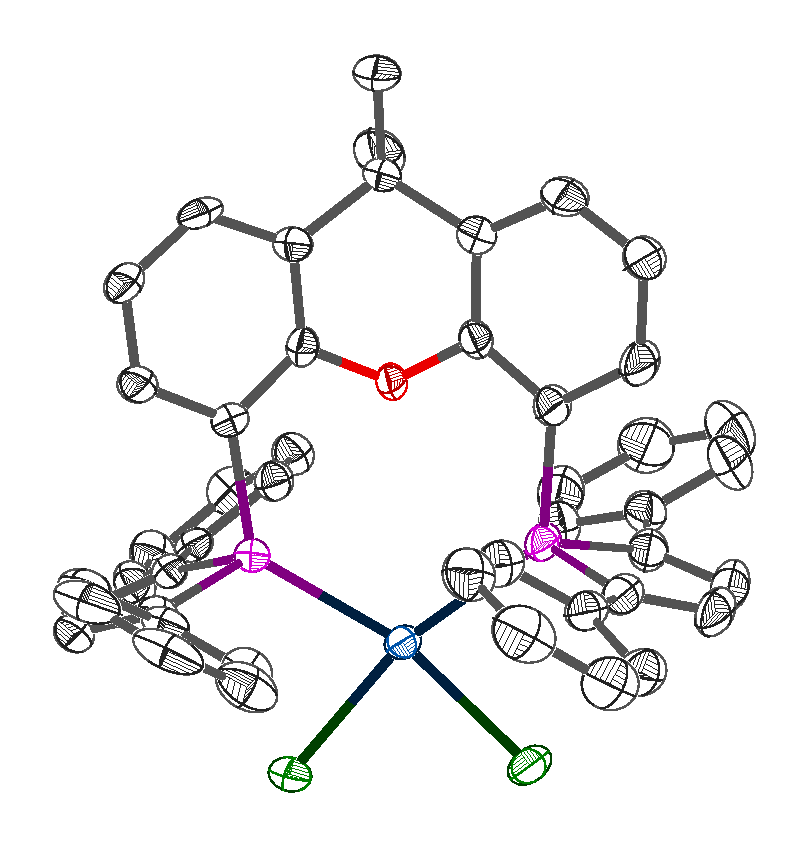
\includegraphics[width=0.8\textwidth]{../Othercrystals/PtCl2/687181.eps}
                \caption{113.39(3)\degrees{}\cite{Mora2008}}
                \label{PtCl2NHC}
        \end{subfigure}
        \\
        \begin{subfigure}[b]{0.6\textwidth}
                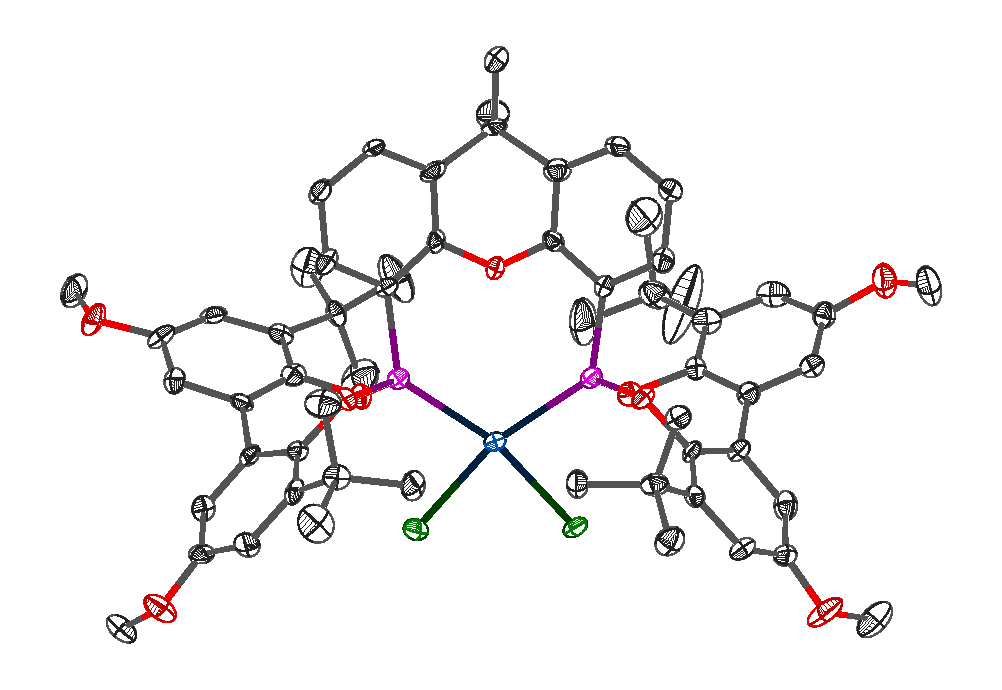
\includegraphics[width=\textwidth]{../Othercrystals/PtCl2/220613.eps}
                \caption{113.43(6)\degrees{}\cite{Vlugt2003}}
                \label{PtCl2}
        \end{subfigure}
        \caption[X-ray crystal structures of complexes of the type [Pt\ce{Cl2}(xantphos){]}]{X-ray crystal structures of complexes of the type [Pt\ce{Cl2}(xantphos)].  The P-Pt-P angle is indicated.}
        \label{crystal:otherPtCl2}
\end{figure}

The angle of the coordination plane relative to the backbone of the [Pt\ce{Cl2}(xant\-phos)] complexes appears to be related to the bite-angle.  The three xantphos complexes with bite-angles of 99--100\degrees{} (Figure \ref{crystal:otherPtCl2side}) have a coordination plane that is almost perpendicular to the plane of the xantphos backbone (105.90(12)\degrees{}, 74.42(13)\degrees{} and 77.0(4)\degrees).  In contrast, the two xantphos complexes with bite-angles of 113.39(3) and 113.43(6)\degrees{} show coordination planes that are in-line with the xantphos backbone (176.9(2)\degrees{} and 178.63(10)\degrees{}).  This is likely the result of the cyclic bulky substituents on the phosphorus atoms of these complexes.  In contrast, the [Pt(\tButhixantphos)\ce{Cl2}] complex, with a much larger bite-angle of 151.722(15)\degrees{}, shows an angle of 140.48(5)\degrees{} between the P-Ar bonds and the Pt coordination plane.  This shows the marked difference between the [Pt(\tButhixantphos)\ce{Cl2}] complex and the other [Pt\ce{Cl2}(xantphos)] complexes.  The change in the position of the coordination plane relative to the backbone is due to the bulky \tBu-substituents causing a distorted \trans{} coordination geometry.  In all of the xantphos crystal structures the ligand backbone is bent, which is clear in the side-on view (Figures \ref{crystalthixantphosplatinumdichlorideside} and \ref{crystal:otherPtCl2side}).  This bending results in a concave face that is less sterically hindered than the convex face.  Hence the coordination plane tilts such that the chloride on the concave face is closer to the backbone than the chloride on the convex face.  

\begin{figure}[htbp]
        \centering
        \begin{subfigure}[b]{0.3\textwidth}
                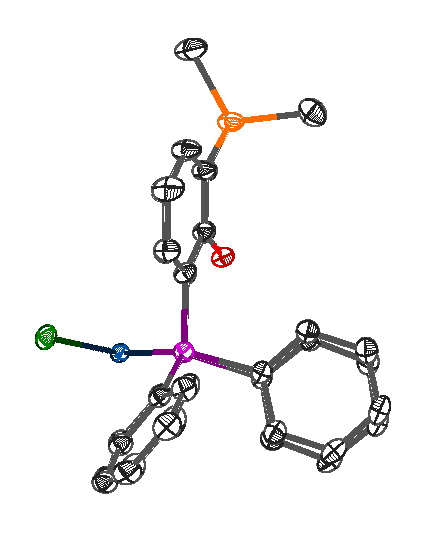
\includegraphics[width=\textwidth]{../Othercrystals/PtCl2/630063side.eps}
                \caption{105.90(12)\degrees{}\cite{Duren2007}}
                \label{PtCl2SiPhside}
        \end{subfigure}%
        ~ 
        \begin{subfigure}[b]{0.25\textwidth}
                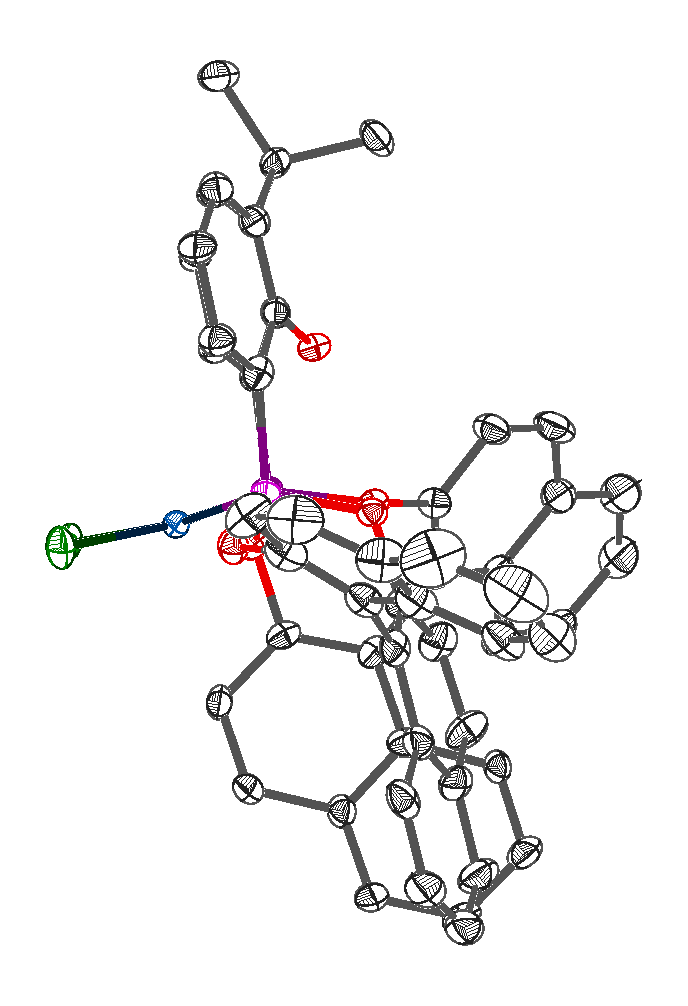
\includegraphics[width=\textwidth]{../Othercrystals/PtCl2/295949side.eps}
                \caption{74.42(13)\degrees{}\cite{Duren2006}}
                \label{PtCl2BINAPside}
        \end{subfigure}
        ~
        \begin{subfigure}[b]{0.3\textwidth}
                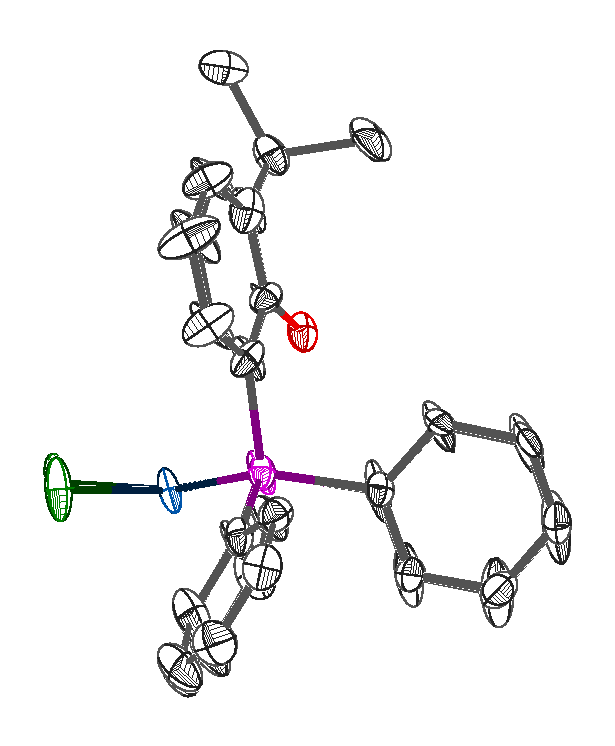
\includegraphics[width=\textwidth]{../Othercrystals/PtCl2/730506side.eps}
                \caption{77.0(4)\degrees{}\cite{Niksch2010}}
                \label{PtCl2Cyside}
        \end{subfigure}%
        \\
        \begin{subfigure}[b]{0.4\textwidth}
                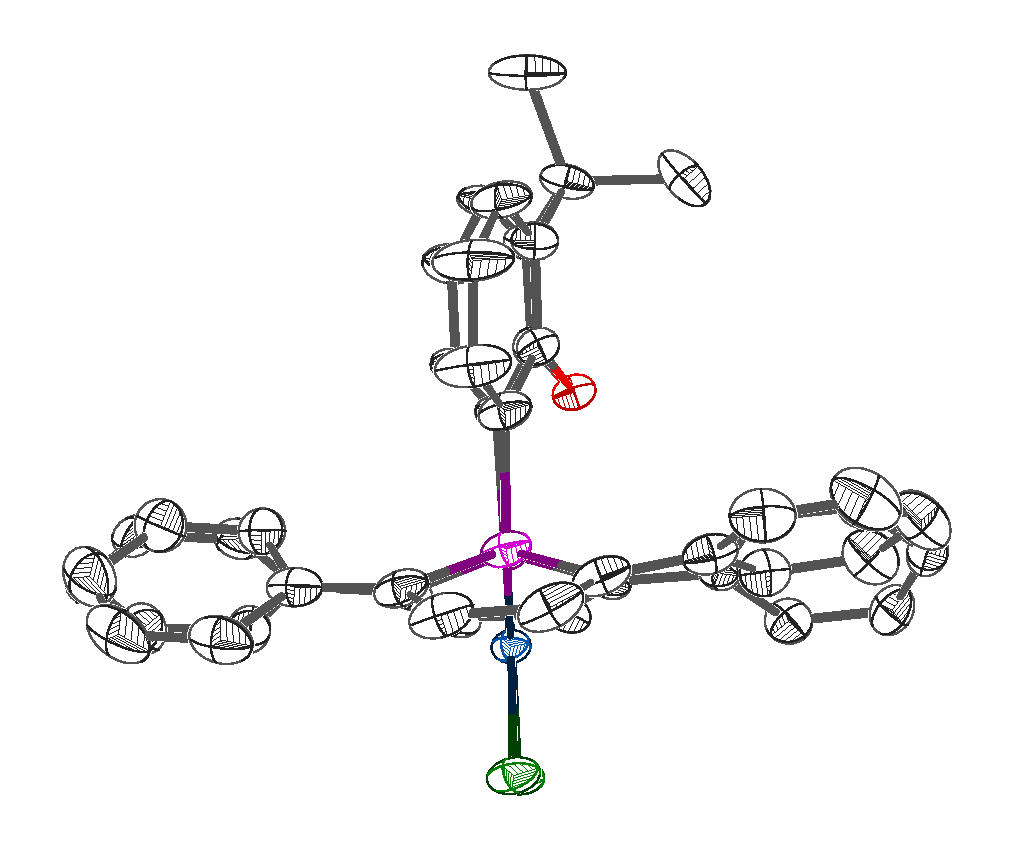
\includegraphics[width=0.9\textwidth]{../Othercrystals/PtCl2/687181side.eps}
                \caption{178.63(10)\degrees{}\cite{Mora2008}}
                \label{PtCl2NHCside}
        \end{subfigure}
        ~
        \begin{subfigure}[b]{0.4\textwidth}
                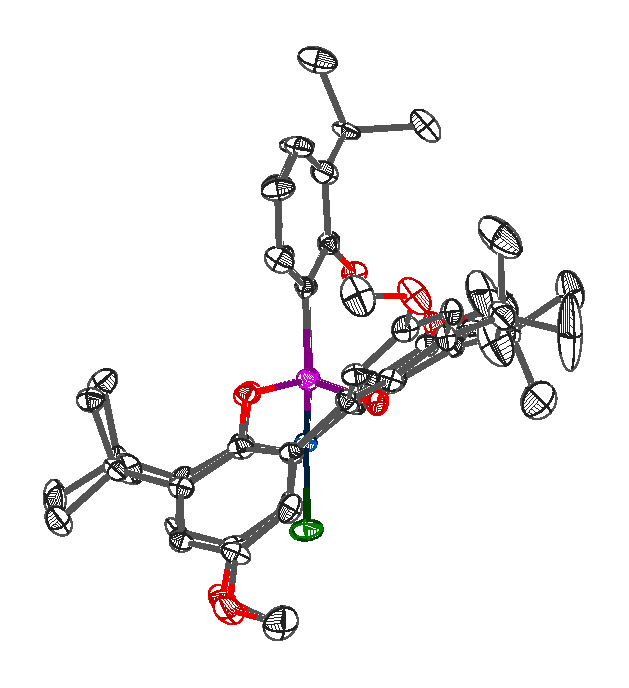
\includegraphics[width=\textwidth]{../Othercrystals/PtCl2/220613side.eps}
                \caption{176.9(2)\degrees{}\cite{Vlugt2003}}
                \label{PtCl2side}
        \end{subfigure}
        \caption[Side-on view of X-ray crystal structures of complexes of the type [Pt\ce{Cl2}(xantphos){]}]{Side-on view of X-ray crystal structures of complexes of the type [Pt\ce{Cl2}(xantphos)] showing the coordination plane relative to the xantphos backbone. The value of the angle between the mean coordination plane and the P-backbone bond is given beneath each structure.}
        \label{crystal:otherPtCl2side}
\end{figure}

While the geometry of [Pt(\tButhixantphos)\ce{Cl2}] is unusual when compared to other platinum complexes, there are 805 bis-phosphine dichloridopalladium complexes in the \gls{CSD}, with 18 of these having P-Pd-P angles between 150 and 167\degrees{} (no platinum complexes of this type with a bite-angle in this region have been reported).\cite{Allen2002}  All of these complexes include diphosphine ligands, indicating the importance of the ligand in controlling the coordination geometry of the complex.  Of particular interest is the structure of [Pd(\tBuxantphos)\ce{Cl2}].\cite{Allen2002}  This structure has three distinct molecules of [Pd(\tBuxantphos)\ce{Cl2}] within the unit cell, with bite-angles of 152.30(4), 152.91(4) and 152.83(4)\degrees.  These are all slightly larger than the P-Pt-P angle in [Pt(\tButhixantphos)\ce{Cl2}], which is expected due to the larger natural bite-angle of \tBuxantphos{}.  In other respects the crystal structures are very similar.  

The bond lengths for the coordinating atoms in [Pt(\tButhixantphos)\ce{Cl2}] are all close to the average values determined from the Cambridge Crystallographic Data Centre (Table \ref{table:crystalthixantphosplatinumdichloride:lengths}).  The Pt-O distance is 2.8016(11) \si{\angstrom}, significantly longer than the average reported Pt-O bond length (2.053 \si{\angstrom}) indicating that there is no interaction between the two atoms.  However, this is shorter than the five other complexes with xantphos derived backbones (3.174-3.466 \si{\angstrom}) indicating that there is a relationship between the bite-angle of the diphosphine and the proximity of the oxygen atom.  

%The choice of starting material and conditions was shown to be very important to the success of the reaction between \tButhixantphos{} and common platinum dichloride starting materials (Table \ref{table:dichlorideprecursors}).  In most cases the reactions required heating.  The only exception to this was with using \ce{[Pt(1,5-hexadiene)Cl2]} in \ce{CH2Cl2} where \fixme{some amount} of the product was observed after 24 hours at room temperature.  The reactions with \cis{} and \trans{}-\ce{[Pt(MeCN)2Cl2]} showed no evidence for any platinum containing product.  The only product observed was the protonated \tButhixantphos{} ligand, occurring due to the formation of hydrochloric acid in the solvent (see section \ref{section:ligands:basicity} for further discussion of the Bronsted basicity of \tButhixantphos).  The only starting materials which displayed significant conversion to a dichloride product were \trans\ce{[Pt(tBuCN)2Cl2]} and \ce{[Pt(1,5-hexadiene)Cl2]}.  Some conversion was observed using \ce{[Pt(SEt2)2Cl2]}, however this was very limited and was only apparent after 28 days at elevated temperature.  
%
%The difference in the reactivity of these molecules is inversely correlated with the bonding strength of these ligands to platinum(II).  Alkenes coordinate through their \fixme{pi}-electrons to the metal centre which is stabilised by back-donation from the metal d-orbitals into an empty \fixme{pi*} orbital on the alkene.  This back-donation is reduced on platinum(II) compared to platinum(0) thus making alkenes readily displaced on platinum(II).  The diethyl sulfide molecule has been reported as able to displace 1,5-cyclooctadiene \fixme{COD} from platinum which in turn is able to displace 1,5-hexadiene.  Furthermore, previous work in our research group has shown that thioethers can readily displace alkene ligands on platinum, whilst ethene does not displace thioethers.  Thus the diethyl sulfide ligand coordinates more strongly to the platinum than 1,5-hexadiene does, hence the reaction is much slower with \ce{[Pt(SEt2)2Cl2]}.  
%
%Nitriles and nitrogen donors in general are also generally considered weakly coordinating ligands on platinum.  Acetonitrile and \tBu-nitrile have been shown to displace one half of a 1,5-cyclooctadiene molecule on iridium (the other half of the 1,5-cyclooctadiene undergoes metallation to form a \fixme{sigma}-bonded \fixme{weird cyclooctadiene thing} and a hydride)\cite{Hermann2002} and acetonitrile in \trans-\ce{[Pd(MeCN)2Cl2]} has been displaced by a number of different ligands including dimethyl sulfide.\cite{Davies1981}  This indicates that the nitrile ligands coordinated more strongly than alkene ligands (such as 1,5-hexadiene) but less strongly than thioether ligands (such as diethyl sulfide).  Furthermore in the case of the iridium complexes the \tBu-nitrile ligand could be readily displaced by the acetonitrile.\cite{Hermann2002}  Hence one would predict a series of ease of displacement with diethyl sulfide < acetonitrile < \tBu-nitrile < 1,5-hexadiene.  However, while \tBu-nitrile and diethyl sulfide showed some reaction (although it was after 28 days for diethyl sulfide), no platinum containing products were observed either the \cis{} or \trans{} acetonitrile complexes.  The reaction with the \cis-\ce{[Pt(MeCN)2Cl2]} starting material was only studied for 72 hours at 20 \degC, and it is possible that this may have reacted given sufficient time and heat.  With \trans-\ce{[Pt(MeCN)2Cl2]} the only product observed after 7 days at 50 \degC{} was the protonated ligand.  Thus indicating that although the nitrile ligands may be more labile than the diethyl sulfide ligand, the light-promoted formation of hydrochloric acid in the samples was more rapid than the reaction between the platinum precursor and the \tButhixantphos{} ligand.  
%
%Interestingly although the reactions between \tButhixantphos{} and the nitrile precursors; \cis{} and \trans{}-\ce{[Pt(MeCN)2Cl2]}, and \ce{[Pt(tBuCN)2Cl2]}, resulted in the formation of the protonated \tButhixantphos{} the reaction with \ce{[Pt(tBuCN)2Cl2]} continued beyond this point to form another complex which is not the \ce{[Pt(\tButhixantphos)Cl2]} complex.  This new complex appears in the \phosphorus{} NMR spectrum at 45.7 ppm with platinum satellites of 2354 Hz.  There is no evidence in the \proton{} or \carbon{} NMR spectra for coordination of the \tBu-nitrile ligand.  For reasons that will be discussed further shortly the \ce{[Pt(\tButhixantphos)Cl2]} complexes undergo solvent dependent dissociation of one of the chloride ions to form \ce{[Pt(\tButhixantphos)Cl]Cl} complexes.  The presence of the uncoordinated \tBu-nitrile may have changed the properties of the \ce{CDCl3} sufficiently that we are able to observe this dissociation when otherwise we normally would not in chloroform.
%
%\begin{sidewaystable}[htp]
%\caption[Reaction of tBu-thixantphos with various platinum dichloride precursors]{Reaction of tBu-thixantphos with various platinum dichloride precursors}
%\vspace{1em}
%\label{table:dichlorideprecursors}
%\small
%\begin{center}
%\begin{tabular}{l l l l l}
%	\toprule
%	~~Starting Material	&Solvent	&Temperature	&Time	&Yield (by NMR)\\
%	\midrule		
%~~Pt(hex)Cl2			& \ce{C6D6}		& 20 \degC	& 4 hours		& No reaction	\\%1052
%~~Pt(hex)Cl2			& \ce{CH2Cl2}		& 20 \degC	& 24 hours	& 24\%{} complex, 32.5\%{} protonated ligand and 43.5\%{} free ligand \\ %4013
%~~Pt(hex)Cl2			& \ce{C6D6}		& 40 \degC	& 72 hours	& 74.9\% Product, 25.1\% free ligand \\
%~~Pt(hex)Cl2			& Toluene			& 50 \degC	& 72 hours	& 100\% Product \\%4011, 4013, 4028
%~~Pt(hex)I2			& \ce{CH2Cl2}		& 20 \degC	& 24 hours	& 49.1\% \tButhixantphos H+, 50.9\% free ligand	\\ %1072
%~~Pt(hex)I2			& \ce{CH2Cl2}		& 20 \degC	& 20 days		& 93.6\% \tButhixantphos H+, 6.4\%, free ligand	\\
%~~PtCl2(SEt2)2			& \ce{C6D6}		& 20 \degC	& 24 hours	& No reaction	\\%1053
%~~PtCl2(SEt2)2			& \ce{C6D6}		& 40 \degC	& 7 days		& 0.4\% Product, 99.6\% free ligand 	\\%1053
%
%~~PtCl2(SEt2)2			& \ce{C6D6}		& 60 \degC	& 4 days	& 3.1\% product, 96.9\% free ligand		\\%1053
%~~PtCl2(SEt2)2			& \ce{C6D6}		& 60 \degC	& 28 days		& 6.7\% product, 92.4\% free ligand\\ %1053
%~~PtCl2(MeCN)2 -cis	& \ce{CD2Cl2}		& 20 \degC	& 72 hours	& 16.2\% \tButhixantphos H+, 83.8\% free ligand	\\%1054
%~~PtCl2(MeCN)2 - trans	& \ce{CDCl3}		& 20 \degC	& 24 hours	& No reaction\\ %1067
%~~PtCl2(MeCN)2 - trans	& \ce{CDCl3}		& 50 \degC	& 7 days		& 33.3\% \tButhixantphos H+, 66.7\% free ligand \\ %1067
%~~PtCl2(MeCN)2 - trans	& \ce{CDCl3}		& 50 \degC	& 21 days		& 25.3\% product, 31.7\% \tBuxantphos H+, 43.0\% free ligand \\
%~~PtCl2(tBuCN)2 - trans	& \ce{CDCl3}		& 20 \degC	& 24 hours	& 8.9\% \tButhixantphos H+, 91.1\% free ligand \\ %1070
%~~PtCl2(tBuCN)2 - trans	& \ce{CDCl3}		& 50 \degC	& 24 hours	& 24.4\% \tButhixantphos H+, 75.6\% free ligand \\ %1070
%~~PtCl2(tBuCN)2 - trans	& \ce{CDCl3}		& 50 \degC	& 7 days 		& 18.2\% product, 32.5\% \tButhixantphos H+ and 49.3 \% free ligand\\%1070
%~~PtCl2(tBuCN)2 - trans	& \ce{CDCl3}		& 50 \degC	& 21 days		& 41.9\% product at 45 ppm, 50.7\% \tButhixantphos H+, 7.4\% free ligand \\ %1070
%%~~K2[PtCl4]			&		&		&		&	\\
%	\bottomrule{}
%\end{tabular}
%\end{center}
%\end{sidewaystable}
%
%%No platinum complexes with observed in the \phosphorus{} NMR spectrum upon reaction was observed with either \cis{} or \trans{}-\ce{[Pt(MeCN)Cl2]}.  
%
%The reaction with platinum dichloride starting materials formed exclusively the \emph{trans}-dichloride platinum diphosphine complexes regardless of the geometry of the starting material and no evidence for \emph{cis}-chelation was observed at any point throughout the reaction.  \fixme{reference}  This is highly unusual for diphosphine ligands.  The ability to form \emph{trans}-chelates is rare for diphosphines and those that can form \trans-spanning complexes typically form a mixture of \emph{cis} and \emph{trans}-geometries.\cite{Freixa2008}  Xantphos itself almost exclusively forms \emph{cis} chelates and the few examples of \emph{trans}-chelation of xantphos that do exist are unstable or form as mixtures with the \emph{cis}-chelates. \fixme{references and structures?}

The \proton{} and \carbon{} NMR spectra of \trans-[Pt(\tButhixantphos)\ce{Cl2}] in \ce{C6D6} show two different sets of \tBu{} carbon and proton resonances.  One of the sets appears as clearly resolved virtual triplets for both carbon environments and the proton environment.  The other set has a well resolved virtual triplet for the quaternary carbon, whereas the other carbon and the proton signal are broad singlets.  The reason for the appearance of two different \tBu{} environments is apparent from the solid-state structure (Figures \ref{crystalthixantphosplatinumdichloride} and \ref{crystalthixantphosplatinumdichlorideside}).  The backbone of the \tButhixantphos{} ligand is bent, resulting in a concave and a convex side.  If the ligand is not inverting in solution then this will result in two different \tBu{} environments: the two on the concave side, and the two on the convex side.  The broadness that is observed for the methyl groups in one of the sets may be due to the steric constraints of this structure.  

The \trans-[Pt(\tButhixantphos)\ce{Cl2}] complex showed a solvent dependent NMR spectrum.  In \ce{C6D6} a single sharp peak was observed at 32.9 ppm (\JPtP = 2700 Hz) in the \phosphorus{} NMR spectrum.  However, in acetone-\ce{d6} this peak became very broad, at 35 ppm, while in \ce{CD2Cl2} or \ce{CDCl3} the peak shifted to 46.4 ppm.  The colour of the complex changes dramatically depending on the solvent.  In the solid state the crystals have been determined to be \trans{}-[Pt(\tButhixantphos)\ce{Cl2}] without any solvent of crystallisation and are deep red in colour.  Benzene and toluene solutions retain this colour.  However, acetone solutions are orange, while in chloroform or dichloromethane the solution is yellow.  Although colour changes for systems with solvent interactions or strong intermolecular interactions are well-known this is unlikely to be the case here.  Instead it is likely that solvent-dependent coordination is occurring.  In non-polar solvents such as benzene and toluene [Pt(\tButhixantphos)\ce{Cl2}] is present.  However, polar solvents like acetone or chloroform are more likely than benzene or toluene to stabilise charged species.  Hence, in polar solvents it is proposed that one of the chloride ligands dissociates and the ether oxygen associates to form [Pt(\tButhixantphosk)Cl]Cl (Scheme \ref{scheme:chloridedissociation}).  In acetone the broadness of the spectrum combined with the intermediate colour likely indicates the rapid interconversion of the complexes.  

\begin{scheme}[ht]
\begin{center}
\vspace{0.5cm}
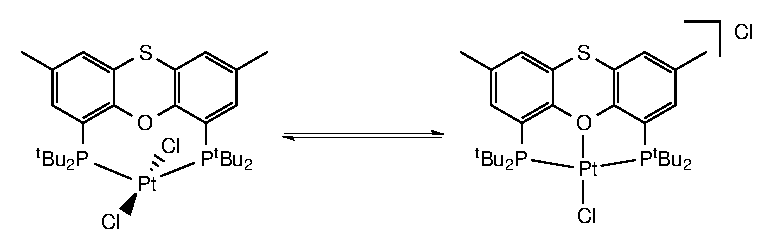
\includegraphics{../Schemes/Chloridedissociation.eps}
\caption[Equilibrium between [Pt(\tButhixantphos)\ce{Cl2{]}} and Pt(\tButhixantphos)Cl{]}Cl]{Equilibrium between [Pt(\tButhixantphos)\ce{Cl2]} and Pt(\tButhixantphos)Cl]Cl.}
\vspace{0.2cm}
\label{scheme:chloridedissociation}
\end{center}
\end{scheme}
\vspace{0.2cm}

To test the chloride dissociation theory, the [Pt(\tButhixantphos)\ce{Cl2}] complex was dissolved in acetone and reacted with ammonium hexafluorophosphate.  The solution changed colour over 30 minutes from deep orange to yellow, and a precipitate of ammonium chloride formed.  The product appeared at 46.4 ppm (\JPtP = 2347 Hz) in the \phosphorus{} NMR spectrum with an associated septet at -144.5 (\JPF{} = 710.6) ppm indicative of \ce{PF6}.  The value of \JPtP{} had decreased from the dichloride complex by 353 Hz, which may be the result of changes in the coordination geometry of the platinum centre.  A shift of the signal in the \carbon{} NMR spectrum for the O-\emph{ipso} carbon occurred from 155.8 ppm to 157.4 ppm, indicative of the oxygen coordinating to the metal centre.


%The relationship between these two compounds was further studied by variable temperature \phosphorus NMR analysis \fixme{figure?}.  A sample of \ce{[Pt(tBu-thixantphos)Cl2]} in \ce{CD2Cl2} was analysed down to -80 \degC.  At room temperature a single broad resonance at 32.9 ppm was observed.  Upon cooling down to -20 \degC this resolved into a single sharp peak, however cooling further led to the conversion of this dichloride into the monochloride appearing at 46.4 ppm.  The mono chloride became the major product below approx -60 \degC.  This may be due to the steric influence of the chlorides and the diphosphine.  At room temperature and above the complex has sufficient energy to exchange between the dichloride and monochloride complexes resulting in a single broad peak.  However upon lowering the temperature the dichloride is preferred.  Lowering further preferences the monochloride.  This effect is likely sterics, at the lower temperature the complex has less energy to move and thus prefers a structure with sufficient space to for all of the ligands around the platinum.   \fixme{I don't actually think I did this?}



%The choice of starting material was shown to be very important to the speed of the reaction.  A large number of different starting materials were investigated with nitrile, thioether, alkene and chloride leaving groups.  An overview of reaction conditions and results are given in Table \ref{table:dichlorideprecursors}.  The fastest of the dichloride materials investigated was \ce{[Pt(hex)Cl2]} this starting material is often used as alkene bind weakly to platinum and are readily displaced by phosphines.  Interestingly although this is a \emph{cis}-dichloride and the product is a \emph{trans}-dichloride the \ce{[Pt(hex)Cl2]} reacted much faster than any of the other precursors.  This is likely a result of the ease of substitution of platinum alkenes relative to platinum nitriles or thioethers.  \fixme{try Zeises dimer?, remove this paragraph}

%There are two major pathways that have been reported for the \cis{}-\trans{} isomerisation of platinum(II) square-planar complexes.  Given that [Pt\ce{Cl2}(\tButhixantphos)] is a 16-electron complexes the isomerisation can proceed through either an associative or a dissociative mechanism (Scheme \ref{Dissociationmechanism}).  Although [Pt(\tButhixantphos)\ce{Cl2}] is an electron deficient 16-electron complex and transition metal complexes generally follow the 18-electron rule, \cis{}-\trans{} isomerisation of platinum(II) square-planar complexes has typically been regarded as following a dissociative pathway.  In this case a chloride ligand would dissociate, followed by the \tButhixantphos{} ligand rearranging to a \trans{} geometry.  This intermediate would likely be stabilised by the reversible coordination of the oxygen in the backbone of the \tButhixantphos{} ligand.  The oxygen could then dissociate allowing for the chloride ligand to recoordinate to generate the \trans{} product.  

%\begin{scheme}[hp]
%\begin{center}
%\vspace{0.5cm}
%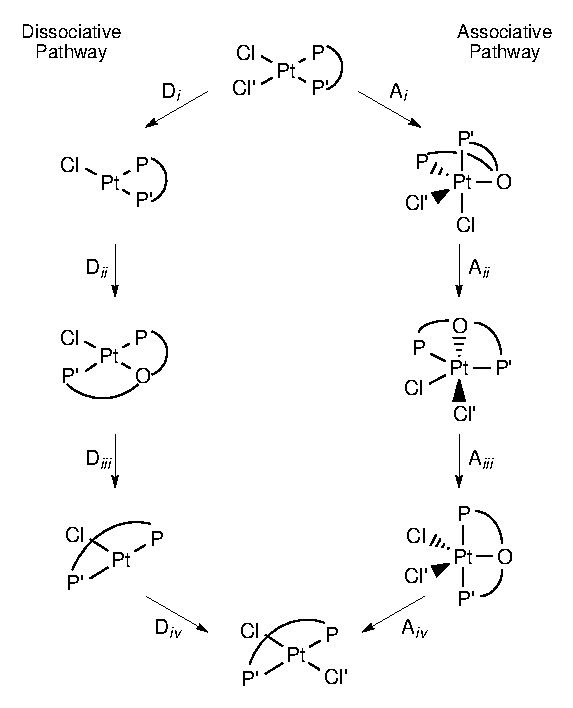
\includegraphics{../Schemes/Dichloridemechanism.eps}
%\caption[\cis-\trans{} Isomerisation pathways for [Pt\ce{Cl2}(\tButhixantphos){]} complexes]{\cis-\trans{} isomerisation pathways for [Pt\ce{Cl2}(\tButhixantphos){]} complexes.  D\sub{i}: dissociation of a chloride ligand, D\sub{ii}: association of the \POP{} oxygen, D\sub{iii}:dissociation of the \POP{} oxygen, D\sub{iv}: association of a chloride ligand.  A\sub{i}: association of the \POP{} oxygen, A\sub{ii}: first Berry pseudo-rotation, A\sub{iii}: second Berry pseudo-rotation, A\sub{iv}: dissociation of the \POP{} oxygen.}
%\vspace{0.2cm}
%\label{Dissociationmechanism}
%\end{center}
%\end{scheme}
%\vspace{0.2cm}

%However, the majority of dichloridoplatinum(II) complexes that have been observed to undergo \cis{}-\trans{} isomerisation do no have the possibility of an intramolecular hemilabile group which could take part in the reaction.  Previous studies of the isomerisation of [Pd\ce{Cl2(PPh3)2}] in THF have shown that a molecule of THF is able to coordinate to the metal promoting an associative mechanism.  In the case of [Pt(\tButhixantphos)\ce{Cl2}] the ether bridge in the backbone could act in the place of a THF molecule and will likely be more rapid due to the intramolecular nature of the reaction.  In this case, the mechanism involves coordination of the oxygen followed by two Berry pseudo-rotations resulting in a complex with the phosphorus atoms of the \tButhixantphos{} ligand occupying both of the axial sites, and the oxygen donor occupying an equatorial site.  From this position the oxygen could readily dissociate to form the \trans-[Pt(\tButhixantphos)\ce{Cl2}] product.

%The presence of the ether bridge of the \tButhixantphos{} ligand which is able to act as an intramolecular donor should promote the associative pathway.  However, the steric bulk and the strong electron donation of the \tBu{} substituents on the phosphorus atoms would likely promote the dissociative pathway.  Several examples of five or six-coordinate rhodium complexes with \tButhixantphos{} acting as a pincer ligand were described in the rhodium chapter \ref{ch:rhodium} indicating that the steric bulk of the ligand does not preclude the formation of species with a higher coordination number.  One of the intermediates in the dissociative pathway is the [Pt(Cl)(\POP-\tButhixantphos)]Cl complex which forms in acetone, chloroform and to some extent in dichloromethane.  However, although we observe this as a product of the reaction this does not necessarily indicate that the associative pathway is not contributing to some extent.

\subsection[Reactions with \texorpdfstring{[Pt\ce{Cl2}(\acrshort{hex}){]}} P]{Reactions of \texorpdfstring{[Pt\ce{Cl2}(hex){]}} P with \tBusixantphos{} and \tBuxantphos{}}

Several starting materials were investigated for the synthesis of \trans-[Pt(\tButhixantphos)\ce{Cl2}]. The best results occurred using \ce{[PtCl2}(\acrshort{hex})], which proceeded in \ce{C6D6} at 40 \degC{} showing 75\% conversion after 72 hours, or in toluene at 50\degC{} with 100\% conversion in the same time.  Due to the success of these conditions over other choices of starting material, temperature, and solvent, the synthesis of analogous \trans-[Pt\ce{Cl2P2}] complexes with \tBusixantphos{} and \tBuxantphos{} was attempted using \ce{[PtCl2}(\acrshort{hex})], in toluene at 50 \degC{}.  

The reaction between \tBuxantphos{} and \ce{[PtCl2}(\acrshort{hex})] proceeded as expected.  After 72 hours at 50\degC{} in toluene an orange solid was isolated which was further purified by recrystallisation, \emph{via} inwards diffusion of diethyl ether into a dichloromethane solution of the product.  The \phosphorus{} NMR spectrum showed one major product at 32.4 ppm (\JPtP{} = 2721 Hz, \ce{C6D6}).  The downfield shift of the peak in the \phosphorus{} NMR spectrum is indicative of complexation.   The value of 2721 Hz is consistent with a phosphorus \trans{} to another phosphorus donor, rather than \trans{} to a chloride ligand.\cite{Rigamonti2010, Appleton1978, Pregosin1980}  The position of the peak and the value of the one-bond platinum-phosphorus coupling constant are very similar to those for \trans-[Pt(\tButhixantphos)\ce{Cl2}] (32.9 ppm, \JPtP{} = 2700 Hz), suggesting the formation of an analogous product, \trans-[Pt(\tBuxantphos)\ce{Cl2}].

The reaction between \tBusixantphos{} and \ce{[PtCl2}(\acrshort{hex})] was not straightforward.  After 72 hours at 50\degC{} the reaction contained unreacted \tBusixantphos{} (53.4\%), [(\tBusixantphos)\ce{H]+} (22.8\%), and a platinum complex.  Although the protonation of \tButhixantphos{} did occur in a number of the reactions with various different [Pt\ce{Cl2L2}] starting materials, this side-reaction was only observed when chlorinated solvents were used.  Hence the formation of [(\tButhixantphos)\ce{H]+} can be attributed to the formation of small amounts of hydrochloric acid due to the UV-catalysed degradation of chlorinated solvents.  However, the formation of [(\tBusixantphos)\ce{H]+} also occurred in toluene and \ce{C6D6}.  There are two possible proton sources, either small amounts of water which may have entered the reaction, or reaction with the surface of the glassware.  The solvents were all degassed and dried over molecular sieves in accordance with Armarego and Chai.\cite{Purificationbook}  This should result in a water concentration of 0.9 ppm for toluene, which is insufficient to account for the conversion.\cite{Williams2010}  Furthermore, the \tBusixantphos{} ligand synthesis involves a dichloromethane/water liquid/liquid separation and no protonation was evident in the \proton{} or \phosphorus{} NMR spectra of the \tBusixantphos{} ligand after this step.  This makes it unlikely that water is the proton source in this reaction.  

Analysis of the \tBuxantphos{} selenides (Section \ref{section:selenides}) showed that \tBusixantphos{} is the most basic of all of the ligands with a \pKb{} of 5.67 compared to 6.90 and 6.72 for \tButhixantphos{} and \tBuxantphos{} respectively.  Hence the \tBusixantphos{} ligand is significantly more susceptible to protonation, leading to the observed difficulties.  The \tBusixantphos{} ligand has the smallest calculated bite-angle of the three ligands (Section \ref{section:biteangle}) which would result in additional strain when forming the \trans-[Pt(\tBusixantphos)\ce{Cl2}] complex compared to the other two ligands.  The reaction with \tButhixantphos{} requires 72 hours at 50 \degC{} to reach completion.  It is likely that the reaction with \tBusixantphos{} would require additional time or harsher conditions to go to completion.  Hence the formation of \trans-[Pt(\tBusixantphos)\ce{Cl2}] has a larger activation barrier compared with the \tButhixantphos{} or \tBuxantphos{} ligands, making the alternative protonation reaction more likely to occur.  

Despite the significant amounts of [(\tBusixantphos{})\ce{H]+} that formed, one species that displays platinum coupling in the \phosphorus{} NMR spectrum is formed.  This species was not isolated and due to the complexity of the \proton{} and \carbon{} NMR spectra for the reaction mixture these were unable to be fully assigned.  The peak for the  platinum containing species appears in the \phosphorus{} NMR spectrum at 34.7 ppm (\JPtP{} = 2686 Hz, \ce{C6D6}).  The value of \JPtP{} is indicative of a \trans{} arrangement of phosphorus atoms.\cite{Rigamonti2010, Appleton1978, Pregosin1980}  The position of the \phosphorus{} NMR signal and the value of \JPtP{} are similar to the \trans-[Pt(\tButhixantphos)\ce{Cl2}] complex which appears at 32.9 ppm (\JPtP{} = 2700 Hz, \ce{C6D6}).  Based on this evidence the product of the reaction between \tBusixantphos{} and \ce{[PtCl2}(\acrshort{hex})] is \trans{}-[Pt(\tBusixantphos)\ce{Cl2}].  The mass spectrum shows a peak with a consistent mass and isotopic distribution for \ce{[C30H48ClOP2PtSi]+}, which could result from loss of a chloride from \trans-[Pt(\tBusixantphos)\ce{Cl2}].\cite{Henderson1998}


[Pt\ce{Cl2}(xantphos)] complexes have been reported for \Phsixantphos, \Phthixantphos{} and \Phxantphos{}.\cite{Kranenburg1998b}  Unlike the \trans-[Pt(\tBuxantphos)\ce{Cl2}] complexes the \Phxantphos{} complexes form \cis{}-[Pt(\Phxantphos)\ce{Cl2}] with \JPtP{} values over 3600 Hz (Table \ref{table:PtCl2NMR}), indicative of phosphorus \trans{} to a chloride ligand.  The \JPtP{} values for the \trans-[Pt(\tBuxantphos)\ce{Cl2}] complexes are almost 1000 Hz lower, indicative of \trans{} coordination of the phosphorus atoms.  The \cis{} geometries of the \Phxantphos{} complexes have been confirmed by X-ray crystallography of \cis{}-[Pt(\Phsixantphos)\ce{Cl2}]\cite{Duren2007} and \cis{}-[Pt(\Phxantphos)\ce{Cl2}].\cite{Niksch2010}  The pseudo-\trans{} geometry of \trans-[Pt(\tButhixantphos)\ce{Cl2}] has been determined crystallographically (Figure \ref{crystalthixantphosplatinumdichloride}). 

The \proton{} and \carbon{} NMR spectra for all three \trans-[Pt(\tBuxantphos)\ce{Cl2}] complexes display broad signals for the \tBu{} proton and carbon environments.  The NMR spectra of \trans-[Pt(\tButhixantphos)\ce{Cl2}] showed two different sets of \tBu{} peaks.  Based on the crystal structure these were determined to be on the concave or convex side of the bent backbone.  For the \tBuxantphos{} complex the backbone may be inverting on a similar timescale to the NMR spectroscopy.  This results in a single signal for the \tBu{} groups but broadened due to the similar timescale to the NMR analysis.  The \carbon{} NMR signals for the \emph{O}-\emph{ipso} carbon  shifted very slightly upon coordination (less than 1.1 ppm), which indicates that the oxygen atom is not coordinated to the metal centre, consistent with the crystal structure of \trans-[Pt(\tButhixantphos)\ce{Cl2}].  

\begin{table}[htbp]
\caption[Selected NMR data for [Pt(xantphos)\ce{Cl2}{]} complexes]{Selected NMR data for [Pt(xantphos)\ce{Cl2}] complexes.  Values for \Phxantphos{} complexes are in \ce{CDCl3}\cite{Kranenburg1998} and values for \tBuxantphos{} complexes are in \ce{C6D6}.  \carbon{} data for the \Phxantphos{} complexes was not reported ($\Delta\delta$ = $\delta$\sub{complex} - $\delta$\sub{free ligand}). }
\label{table:PtCl2NMR}
\small
\begin{center}
\begin{tabular}{l c c c c c}
\toprule{}
	~~ & \multicolumn{3}{c}{\bfseries{\phosphorus}} & \multicolumn{2}{c}{\bfseries{\carbon{} \emph{O}-\emph{ipso}}}\\
	\cmidrule(lr){2-4} \cmidrule(lr){5-6}
	\bfseries{Diphosphine}&\bfseries{$\delta/$ppm}&\bfseries{$\Delta\delta/$ppm}&\bfseries{\JPtP}&\bfseries{$\delta/$ppm}&\bfseries{$\Delta\delta/$ppm}\\
	\midrule{}
	\PhSixantphos		& 7.6	   & 25.2 & 3663 & &\\
	\PhThixantphos		& 8.4   & 25.7 & 3641 &&\\
	\PhXantphos		& 6.6	   & 24.1 & 3695 & &\\
	\tBuSixantphos 		& 34.7 & 26.3 & 2686 &&\\
	\tBuThixantphos 	& 32.9 & 23.4 & 2700 & 155.8 & -0.1\\
	\tBuXantphos		& 32.4 & 22.2 & 2721 & 157.1 & 1.1\\
	\bottomrule{}
\end{tabular}
\end{center}
\end{table}

The solvent-dependent coordination that was observed in the synthesis of [Pt(\tButhixantphos)\ce{Cl2}] was also observed for [Pt(\tBuxantphos)\ce{Cl2}], and was studied in more depth for this complex.  Selected NMR data for [Pt(\tBuxantphos)\ce{Cl2}] dissolved in \ce{CDCl3}, \ce{CD2Cl2} and \ce{C6D6} are given in Table \ref{table:solventNMR}.  The complex was also analysed in acetone-\ce{d6} however the \proton{}, \carbon{} and \phosphorus{} NMR spectra were very broad likely indicating the rapid interconversion between [Pt(\tBuxantphos)\ce{Cl2}] and [Pt(\tBuxantphosk)Cl]Cl.  The peak in the \phosphorus{} NMR spectrum shifts by around 15 ppm upon changing the solvent from \ce{C6D6} to \ce{CDCl3} or \ce{CD2Cl2}.  The value of \JPtP{} is lower by more than 370 Hz, consistent with coordination of the oxygen to the metal centre.  The pseudo-\trans{} geometry of the \trans-[Pt(\tBuxantphos)\ce{Cl2}] complexes results in significant strain in the \tBuxantphos{} ligands.  Coordination of the oxygen to the metal centre can relieve the strain and allow much larger P-M-P angles to form.  With a larger P-Pt-P angle the phosphorus atoms are closer to a mutually \trans{} configuration.  The closer to \trans{} the atoms become, the greater the influence of the other phosphorus atom and thus the value of \JPtP{}.  

\begin{table}[htbp]
\caption[Selected NMR data for [Pt(\tBuxantphos)\ce{Cl2}{]} and [Pt(\tBuxantphos)Cl{]}Cl]{Selected NMR data for [Pt(\tBuxantphos)\ce{Cl2}{]} and [Pt(\tBuxantphos)Cl{]}Cl ($\Delta\delta$ = $\delta$\sub{complex} - $\delta$\sub{free ligand}).}
\label{table:solventNMR}
\small
\begin{center}
\begin{tabular}{l c c c c c c}
	\toprule{}
	~~ & ~~ & \multicolumn{3}{c}{\bfseries{\phosphorus}} & \multicolumn{2}{c}{\bfseries{\carbon{} 	\emph{O}-ipso}}\\
	\cmidrule(lr){3-5} \cmidrule(lr){6-7}
	\bfseries{Solvent}&\bfseries{Complex}&\bfseries{$\delta/$ppm}&\bfseries{$\Delta\delta/$ppm}&\bfseries{\JPtP}&\bfseries{$\delta/$ppm}&\bfseries{$\Delta\delta/$ppm}\\
	\midrule{}
	\ce{C6D6} & [Pt(\tBuxantphos)\ce{Cl2}] & 32.4 & 22.2 & 2721.0 & 157.1 & 1.1\\
	\ce{CDCl3} & [Pt(\tBuxantphos)Cl]Cl & 47.7 & 37.5 & 2349.6 & 158.5 & 2.7 \\
	\ce{CD2Cl2} & [Pt(\tBuxantphos)Cl]Cl & 47.8 & 37.6	& 2345.3 & 158.8 & 3.0\\
	\bottomrule{}
	\end{tabular}
	\end{center}
	\end{table}
	
The \proton{} and \carbon{} NMR data for [Pt(\tBuxantphos)\ce{Cl2}{]} and [Pt(\tBuxantphos)Cl]Cl all show virtual triplet peaks for the \tBu{} protons and carbons.  This indicates strongly coupled phosphorus atoms, which typically occurs with mutually \trans{} phosphorus atoms.  However, the \carbon{} peak for the \emph{O}-\emph{ipso} carbon in the \tBuxantphos{} ligand shows a shift of only 1.1 ppm (from the free ligand) when in \ce{C6D6}, but a shift ($\Delta\delta$) of 2.7 or 3.0 ppm in \ce{CDCl3} and \ce{CD2Cl2} respectively.  This shift has been observed for a number of rhodium complexes with the \tBuxantphos{} ligands coordinated as tridentate \POP{} pincer ligands (Chapter \ref{ch:rhodium}).  The downfield shift upon coordination of the oxygen is due to the oxygen donating electron density to the metal, which inductively decreases the electron density on the adjacent carbon atoms, resulting in decreased shielding.  

The solvent dependent formation of [Pt(\tBuxantphos)Cl]Cl complexes was confirmed by reaction of [Pt(\tBuxantphos)Cl]Cl and [Pt(\tButhixantphos)Cl]Cl with \ce{NH4PF6}.  [Pt(\tBusixantphos)\ce{Cl2}] could not be isolated and therefore was not investigated for this reaction.  The two complexes react visibly with \ce{NH4PF6}, changing a dichloromethane solution from orange/red to yellow over a one hour period.  The excess \ce{NH4PF6} and \ce{NH4Cl} by-product are readily removed by concentration of the solution and filteration through a plug of alumina.  Selected NMR data is given in Table \ref{table:PF6NMR}.  The \phosphorus{} NMR spectra clearly show the presence of the \ce{PF6} counterion appearing as a septet at -144.5 ppm (\JPF{} = 710.5 Hz) for both \tButhixantphos{} and \tBuxantphos{}.  The \fluorine{} NMR spectra further confirms this with a clear doublet at -73.4 ppm (\JPF{} = 710.6 Hz).

\begin{sidewaystable}[htbp]
\caption[Selected NMR data for [Pt(\tBuxantphos)Cl{]}X complexes]{Selected NMR data for [Pt(\tBuxantphos)Cl{]}X complexes (X = Cl, \ce{PF6}) in \ce{CD2Cl2} ($\Delta\delta$ = $\delta$\sub{complex} - $\delta$\sub{free ligand}).}
\label{table:PF6NMR}
\small
\begin{center}
\begin{tabular}{l c c c c c c c}
	\toprule{}
	~~ & \multicolumn{5}{c}{\bfseries{\phosphorus}} & \multicolumn{2}{c}{\bfseries{\carbon} \emph{O}-ipso}\\
	\cmidrule(lr){2-6} \cmidrule(lr){7-8}
	\bfseries{Complex}&\bfseries{$\delta/$ppm}&\bfseries{$\Delta\delta/$ppm}&\bfseries{\JPtP/Hz} & \bfseries{$\delta/$ppm} & \bfseries{\JPF$/$Hz} & \bfseries{$\delta/$ppm}&\bfseries{$\Delta\delta/$ppm}\\
	\midrule{}
	{[}Pt(\tButhixantphos)Cl]\ce{PF6} & 46.4 & 36.9 & 2347 & -144.5 & 710.5 & 157.4 & 2.1\\
	{[}Pt(\tBuxantphos)Cl]\ce{PF6} & 47.8 & 37.6 & 2350 & -144.5 & 710.4 & 158.8 & 3.0 \\
	{[}Pt(\tBuxantphos)Cl]Cl & 47.8 & 37.6 & 2345 & N/A & N/A & 158.8 & 3.0\\
	\bottomrule{}
\end{tabular}
\end{center}
\end{sidewaystable}

The \proton{} and \carbon{} NMR spectra for the [Pt(\tBuxantphosk)Cl]\ce{PF6} complexes show virtual triplet peaks for all of the \tBu{} environments, indicative of \trans{} coordination of the phosphorus atoms.  The position of the \emph{O}-\emph{ipso} carbon has also shifted relative to both the free ligand and the [Pt(\tBuxantphos)\ce{Cl2}] complexes (Table \ref{table:PF6NMR}).  The shift from the free ligand is in excess of 2.0 ppm, indicative of the decreased shielding of the \emph{O}-\emph{ipso} carbon that occurs upon coordination of the oxygen to a transition metal.  

%======================================================================

\section{Reactions with \texorpdfstring{[\ce{Pd(cod)Cl2}]} P}

Palladium dichloride complexes are ubiquitous in coordination chemistry, the \gls{CSD} contains over 3000 X-ray crystal structures of palladium dichlorides.\cite{Allen2002}  The interest in these complexes is due to their relative ease of synthesis and high reactivity, which enables their wide use as pre-catalysts in a range of different catalytic processes such as the many palladium catalysed cross-coupling reactions.\cite{Tsuji1995}

The reactivity of the \tBuxantphos{} ligands with palladium(II) was explored with a common palladium(II) starting material, [Pd(\acrshort{cod})\ce{Cl2}] (\acrshort{cod} = \acrlong{cod}).  This complex is very similar to the [Pt\ce{Cl2}(\acrshort{hex})] that was used to explore the analogous chemistry with platinum; hexa-1,5-diene and cod are both readily displaced by phosphine ligands. The reactions between the \tBuxantphos{} ligands and [Pd(cod)\ce{Cl2}] were straightforward, producing only one product in all cases, determined to be the \trans-[Pd(\tBuxantphos)\ce{Cl2}] complex (Figure \ref{Palladiumdichloride}).

\begin{scheme}[ht]
\begin{center}
\vspace{0.5cm}
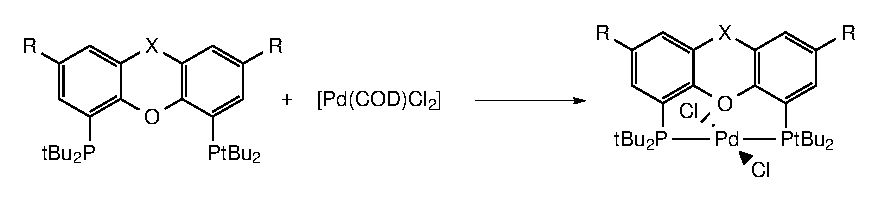
\includegraphics{../Schemes/Palladiumdichloride.eps}
\caption[Synthesis of [Pd(\tBuxantphos)\ce{Cl2}{]}]{Synthesis of [Pd(\tBuxantphos)\ce{Cl2}] complexes. \emph{Reagents and conditions:} (i) [Pd(cod)\ce{Cl2}], toluene, 40\degC{}, 3 days.}
\vspace{0.2cm}
\label{Palladiumdichloride}
\end{center}
\end{scheme}
\vspace{0.2cm}

%Reaction between the tBu-xantphos ligands and \ce{[Pd(COD)Cl2]} was much faster than with any of the platinum dichloride analogues with a dark red species forming rapidly.  A single complex was observed in all cases with single peaks observed in each of the phosphorus NMR spectra.\fixme{give values}  This indicates a symmetrical complex has formed, the \emph{tert}-butyl peaks in the \proton{} NMR spectrum appear as a virtual triplet resonance indicative of \emph{trans}-chelation (Scheme \ref{Palladiumdichloride}).  

Selected NMR data for the \trans-[Pd(\tBuxantphos)\ce{Cl2}] complexes is given in Table \ref{table:PdClNMR}.  The \phosphorus{} NMR spectra each show one singlet, while the \proton{} and \carbon{} NMR spectra display half the total expected number of peaks indicating the presence of a plane of symmetry.  The chemical shift of the \phosphorus{} signal varies between 30.5 and 43.9 ppm for the three complexes.  A downfield shift of this magnitude is consistent with coordination to a transition metal.\cite{Pregosin2012}  In [Pd(\tBuxantphos)\ce{Cl2}] both of the \tBu{} carbon signals and the proton signal appear as virtual triplets, consistent with a \trans{} coordination.  However, the complexes with \tBusixantphos{} and \tButhixantphos{} both have resolved virtual triplets for the \tBu{} protons and quaternary carbon environments, while the terminal carbon signals display some broadening.  The position of the \emph{O}-\emph{ipso} carbon can be indicative of tridentate coordination of the xantphos ligands.  In this case the shift upon coordination ranges from -0.2 to 1.1 ppm.  These are all smaller than would be expected if a chloride had dissociated and a pincer complex had formed.  

\begin{table}[htbp]
\caption[Selected NMR data for [Pd(\tBuxantphos)\ce{Cl2}{]} complexes]{Selected NMR data for [Pd(\tBuxantphos)\ce{Cl2}{]} complexes in \ce{CD2Cl2} ($\Delta\delta$ = $\delta$\sub{complex} - $\delta$\sub{free ligand}).}
\label{table:PdClNMR}
\small
\begin{center}
\begin{tabular}{l c c c c}
	\toprule{}
	~~ & \multicolumn{2}{c}{\bfseries{\phosphorus}} & \multicolumn{2}{c}{\bfseries{\carbon} \emph{O}-ipso}\\
	\cmidrule(lr){2-3} \cmidrule(lr){4-5}
	\bfseries{Diphosphine}&\bfseries{$\delta/$ppm}&\bfseries{$\Delta\delta/$ppm}& \bfseries{$\delta/$ppm} & \bfseries{$\Delta\delta/$ppm}\\
	\midrule
	\tBuSixantphos 		& 46.7	& 38.3	& 165.4	& 1.1 \\
	\tBuThixantphos	& 40.0	& 30.5	& 155.1	& -0.2 \\
	\tBuXantphos		& 54.1	& 43.9	& 156.6	& 0.8	 \\
	\bottomrule{}
\end{tabular}
\end{center}
\end{table}

Unlike the [Pt(\tBuxantphos\ce{)Cl2}] complexes, the [Pd(\tBuxantphos)\ce{Cl2}] complexes do not display solvent dependent coordination.  NMR spectroscopy of the complexes in \ce{CDCl3}, \ce{CD2Cl2}, and \ce{C6D6} showed no substantial changes in either the chemical shift of the \phosphorus{} NMR signal or the \emph{O}-\emph{ipso} carbon.  Selected NMR data for \tBusixantphos{} in different solvents is given in Table \ref{table:PdsolventNMR}.

\begin{table}[htbp]
\caption[Selected NMR data for [Pd(\tBusixantphos)\ce{Cl2}{]}]{Selected NMR data for [Pt(\tBusixantphos)\ce{Cl2}] in different solvents ($\Delta\delta$ = $\delta$\sub{complex} - $\delta$\sub{free ligand}).}
\vspace{1em}
\label{table:PdsolventNMR}
\small
\begin{center}
\begin{tabular}{l c c c c}
	\toprule{}
	~~ & \multicolumn{2}{c}{\bfseries{\phosphorus}} & \multicolumn{2}{c}{\bfseries{\carbon{} 	\emph{O}-ipso}}\\
	\cmidrule(lr){2-3} \cmidrule(lr){4-5}
	\bfseries{Solvent}&\bfseries{$\delta/$ppm}&\bfseries{$\Delta\delta/$ppm}&\bfseries{$\delta/$ppm}&\bfseries{$\Delta\delta/$ppm}\\
	\midrule
	\ce{C6D6} 	& 42.0 & 33.6 & 164.9 & 0.4 \\
	\ce{CDCl3}	& 45.7 & 37.3 & 165.1 & 0.8 \\
	\ce{CD2Cl2}	& 46.7 & 38.3 & 165.4 & 1.1 \\
	\bottomrule{}
	\end{tabular}
	\end{center}
	\end{table}
	
\subsection{Formation of \texorpdfstring{[Pd(\tBuxantphosk)Cl]\ce{PF6}} P Complexes}

The [Pt(\tBuxantphos)\ce{Cl2}] complexes displayed solvent dependent dissociation of one of the chloride ligands.  The pincer complex [Pt(\tBuxantphosk)\ce{Cl]^{+}} was trapped by counterion exchange with \ce{NH4PF6}.  Although the [Pd(\tBuxantphos)\ce{Cl2}] complexes do not display the same solvent dependent coordination, reaction with \ce{NH4PF6} resulted in the analogous [Pd(\tBuxantphos)Cl]\ce{PF6} complexes (Scheme \ref{PdPF6scheme}).  An associated colour change from the deep red dichloride complexes to bright yellow pincer species was observed for all three of the ligands.

\begin{scheme}[ht]
\begin{center}
\vspace{0.5cm}
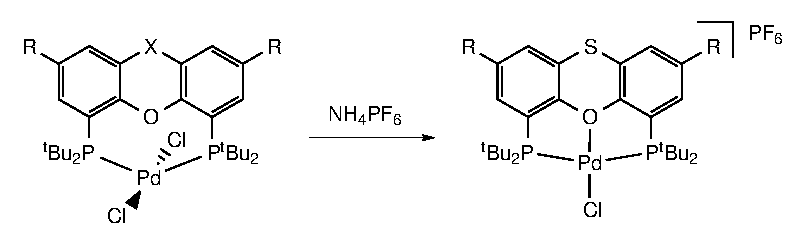
\includegraphics{../Schemes/PdClPF6.eps}
\caption[Synthesis of [Pd(\tBuxantphosk)Cl{]}\ce{PF6}]{Synthesis of [Pd(\tBuxantphosk)Cl{]}\ce{PF6}. \emph{Reagents and conditions:} (i) \ce{NH4PF6}, \ce{CH2Cl2}, 24 hours.}
\vspace{0.2cm}
\label{PdPF6scheme}
\end{center}
\end{scheme}
\vspace{0.2cm}

Selected NMR data of the [Pd(\tBuxantphosk)Cl]\ce{PF6} complexes is given in Table \ref{table:PdPF6NMR}.  The \ce{PF6-} counterion is clearly apparent as a septet in the \phosphorus{} NMR spectrum at -144.5 ppm and a doublet in the \fluorine{} NMR spectrum at -73.4 ppm, indicating a non-coordinating counterion.  The \phosphorus{} NMR signals for the \tBuxantphos{} ligands have all shifted downfield.  The \tBu{} \proton{} and \carbon{} environments for all three complexes now appear as well-resolved virtual triplets indicating \trans{} chelation of the phosphorus atoms.  A reaction has occurred in all cases indicated by a shift in the \phosphorus{} NMR spectrum and the changes of other peaks in the \proton{} and \carbon{} NMR spectra.  Although the change in the chemical shift of the \emph{O}-\emph{ipso} carbon of \tBusixantphos{} from the uncoordinated ligand ($\Delta\delta$) is indicative of oxygen coordination, the values for \tButhixantphos{} and \tBuxantphos{} are not.  This may mean that the oxygen is only very weakly coordinating to the palladium centre and in solution a T-shaped palladium complex is present, or that the complex may be stabilised by other interactions such as weak agostic interactions with the \tBu{} methyl groups or between the palladium atom and the \ce{PF6} counterion.  

\begin{table}[htbp]
\caption[Selected NMR data for [Pd(\tBuxantphos)Cl{]}\ce{PF6} complexes]{Selected NMR data for [Pd(\tBuxantphos)Cl]\ce{PF6} in \ce{CD2Cl2} ($\Delta\delta$ = $\delta$\sub{complex} - $\delta$\sub{free ligand}).}
\label{table:PdPF6NMR}
\small
\begin{center}
\begin{tabular}{l c c c c c c}
	\toprule{}
	~~ & \multicolumn{4}{c}{\bfseries{\phosphorus}} & \multicolumn{2}{c}{\bfseries{\carbon}}\\
	\cmidrule(lr){2-5} \cmidrule(lr){6-7}
	\bfseries{Ligand}&\bfseries{$\delta/$ppm}&\bfseries{$\Delta\delta/$ppm}& \bfseries{$\delta/$ppm} & \bfseries{\JPF$/$Hz} & \bfseries{$\delta/$ppm}&\bfseries{$\Delta\delta/$ppm}\\
	\midrule
	\tBuSixantphos		& 52.4	& 5.7		& -144.5	& 710.3	& 168.4	& 4.1	\\
	\tBuThixantphos 	& 56.4	& 16.4	& -144.5	& 710.5	& 154.9	& -0.4	\\
	\tBuXantphos		& 58.3	& 4.2		& -144.5	& 710.4	& 156.7	& 0.9 \\
	\bottomrule{}
\end{tabular}
\end{center}
\end{table}

%The chloride ligands in the three \ce{[Pd(\tBuxantphos)Cl2]} are relatively weakly, similarly to the platinum case, however no evidence for a monochloride complex is apparent.  Reacting the dichloride complexes with \ce{NH4PF6} in acetone forms an immediate precipitate of \ce{NH4Cl} and the reaction colour changes from a deep red to yellow.\fixme{check that this isn't for the platinum one}  The product has two peaks in the \phosphorus{} NMR spectrum, a septet at -144.5 (710.5 Hz) and a singlet at 56.4 ppm (shifted from 41.9 ppm) indicative of a symmetrical complex and a virtual triplet resonance for the \emph{tert}-butyl peaks.  The O-ipso carbon has a insignificant shift in the \carbon{} NMR spectrum (from 155.1 to 154.9 ppm) indicating that it is likely not coordinated to the palladium.  A large shift occurs for the P-ipso carbon shifting from 123.5 (vt, 12.5 Hz) to 118.7 (vt, 10.8 Hz).  This indicates an increase in the electron density on the carbon and is close to that found for the complex \ce{[Ag(tBu-xantphos)Cl]} (120.9 ppm).  This data confirms the formulation of the complex as \ce{[Pd($\eta^2-$(tBu-xantphos)Cl]PF6}

%======================================================================

\section{Computational Results}

The [Pt(\tBuxantphos)\ce{Cl2}] complexes displayed solvent dependent coordination forming [Pt(\tBuxantphosk)Cl]Cl.  This pincer complex was trapped by the exchange of the counterion using ammonium hexafluorophosphate.  The palladium analogue did not display the same solvent-induced dissociation, although the [Pd(\tBuxantphosk)Cl]Cl complexes could be readily synthesised by reaction with ammonium hexafluorophosphate.  This reactivity, particularly the solvent dependent exchange was investigated further using density functional theory.  The geometries of all structures were optimised and frequencies were calculated using a B3LYP functional\cite{Becke1993, Lee1988, Vosko1980, Stephens1994}, with the def2-TZVP basis set\cite{Andrae1990, Weigend2005}.  The energies of the systems were then calculated with incorporation of a solvent model (SMD).

Structures were optimised for the complexes [M(\tBuxantphos)\ce{Cl2]} and [M(\tBuxantphosk)\ce{Cl]^{+}} (M = Pd, Pt) with the three different \tBuxantphos{} ligands.  The change in energy for the dissociation of a chloride ligand was calculated and the results for each of these reactions are summarised in Figure \ref{comp:dichlorideresults}.  Typical DFT calculations are performed for molecules in the gas phase.  However, this is not always an appropriate description of the system, particularly when conversions between uncharged and charged species are involved as solvent stabilisation can become important.  This is apparent for the dichloride to pincer conversion.  In the gas phase, the systems show that the pincer complexes are around 400 \si{\kilo\joule\per\mole} higher in energy than the corresponding dichloride complex.  This indicates that the reaction would be highly endothermic, although it may still be favoured entropically.

\begin{figure}[htbp]
\begin{center}
\small
\caption[Energy change for conversion from [M(\tBuxantphos)\ce{Cl2}{]} to [M(\tBuxantphos)Cl{]}Cl (M = Pd, Pt)]{Energy change on conversion from the [M(\tBuxantphos)\ce{Cl2}{]} to [M(\tBuxantphos)Cl{]}Cl.}
	\ce{[Pt(diphosphine)Cl2] \rightarrow [Pt(POP)Cl] + Cl-}
	\vspace{1em}
\begin{tabular}{l c c c c c}
	\toprule
	~ & \multicolumn{5}{c}{\bfseries{$\Delta$\emph{E}, \si{\kilo\joule\per\mole}}} \\
	\cmidrule(lr){2-6} 
	~\bfseries{Ligand} & \bfseries{Solvent Free} & \bfseries{\ce{(CH3)2CO}} &\bfseries{\ce{C6H6}}&\bfseries{\ce{CHCl3}} & \bfseries{\ce{CH2Cl2}} \\
	\midrule		
	~\tBusixantphos 	& 393.5	& -2.2	& 150.7 	& 59.0	& 20.4\\
	~\tButhixantphos	& 400.2	& 4.3		& 157.9	& 66.0	& 27.3\\
	~\tBuxantphos		& 384.5	& -14.6	& 140.1	& 47.7	& 8.6\\
	\bottomrule{}
\end{tabular}
\\
\ce{[Pd(diphosphine)Cl2] \rightarrow [Pd(POP)Cl] + Cl-}
	\vspace{1em}
\begin{tabular}{l c c c c c}
	\toprule
	~ & \multicolumn{5}{c}{\bfseries{$\Delta$\emph{E}, \si{\kilo\joule\per\mole}}} \\
	\cmidrule(lr){2-6} 
	~\bfseries{Ligand} & \bfseries{Solvent Free} & \bfseries{\ce{(CH3)2CO}} &\bfseries{\ce{C6H6}}&\bfseries{\ce{CHCl3}} & \bfseries{\ce{CH2Cl2}} \\
	\midrule		
	~\tBusixantphos 	& 397.4	& 0.8		& 155.0 	& 62.7	& 23.7\\
	~\tButhixantphos	& 405.3	& 7.9		& 163.1	& 70.3	& 31.4\\
	~\tBuxantphos		& 391.7	& -7.9	& 83.2	& 55.0	& 15.6\\
	\bottomrule{}
\end{tabular}
\label{comp:dichlorideresults}
\end{center}
\end{figure}

Single point energy calculations for the [M(\tBuxantphos)\ce{Cl2}] and [M(\tBuxantphosk)\ce{Cl]^{+}} in a range of solvents were performed on the structures that had been optimised in the gas phase (Figure \ref{comp:dichlorideresults}).  The results show that the introduction of any solvent reduces the energy required by more than half.  For both the platinum and palladium complexes, the reaction in benzene requires the most energy of any of the solvents studied.  This is consistent with the experimental results, as the platinum complexes are present as [Pt(\tBuxantphos)\ce{Cl2}] in benzene.  For the platinum complexes conversion to [Pt(\tBuxantphosk)Cl]Cl was observed experimentally in chloroform and dichloromethane and the spectrum in acetone was broad, likely indicating some conversion.  Interestingly, the computational results indicate that the lowest energy change occurs for the reaction in acetone, as these values are either close to zero or even negative, while the dichloromethane values are 8.6--27.3 \si{\kilo\joule\per\mole} and the chloroform values are higher still 47.7--66.0 \si{\kilo\joule\per\mole}.  These values do not include entropic effects which are likely to be significant as the disorder is increased.  Although the calculations suggest that the chloride dissociation is an endothermic process, the reactions may be spontaneous due to entropy.  

The results for the palladium complexes show similar overall trends to the platinum complexes (Figure \ref{comp:dichlorideresults}).  However, most of the palladium reactions require slightly more energy than the platinum complexes.  This is consistent with the observation that the reaction is spontaneous for platinum (under certain conditions) while it is not for palladium.  The energy for the palladium complexes in dichloromethane are lower than the energy for the platinum reaction in chloroform, which was observed to be spontaneous experimentally, again indicating that entropy is likely playing a significant role for this reaction.   

%======================================================================

\section[Reactions with Platinum Dimethyl Starting Materials]{Reactions with Platinum Dimethyl Starting\\Materials}

Transition metal alkyl complexes are among the most important organometallic complexes as they can be intermediates in a wide range of catalytic transformations, including polymerisation and carbonylation reactions.\cite{Doherty1999, Veen2002}  The synthesis of isolatable transition metal alkyl complexes is important, as studying their chemistry can give insight into the reactions occurring in catalytic systems.\cite{Moss1996}  Methyl complexes have gained attention in recent years, as protonation of a rho\-dium methyl complex led to a $\sigma$-methane complex which was characterised by NMR spectroscopy.\cite{Bernskoetter2009}  Platinum methyl complexes were investigated as part of this study as the stronger $\sigma$-donor character of the methyl ligand may lead to different reactivity than that of the platinum dichloride complexes.\cite{Appleton1978}

The reactivity of the \tBuxantphos{} ligands with [Pt(\acrshort{hex})\ce{Me2})] was first studied using the \tButhixantphos{} ligand.  \tBuThixantphos{} was combined with [Pt(\acrshort{hex})\ce{Me2]} in an NMR tube in \ce{C6D6} under argon to enable the progress to be followed by NMR spectroscopy.  After 24 hours at room temperature no reaction was observed, so the sample was heated to 60 \degC.  The progress of the sample was monitored at regular intervals.  However, after 28 days at 60 \degC{} no changes were observed.  The \phosphorus{} NMR spectrum showed a single peak indicative of uncoordinated \tButhixantphos{}, and the \proton{} NMR spectrum showed a mixture with [Pt(\acrshort{hex})\ce{Me2]}.  This indicates that the lack of reactivity was not the result of degradation of either the platinum starting material or the \tButhixantphos{} ligand.  

One equivalent of the strong acid \ce{CHPh(SO2CF3)2} was added to the mixture of \tButhixantphos{} and [Pt(\acrshort{hex})\ce{Me2}] in an attempt to protonate the platinum complex and remove one of the methyl ligands as methane, thus forming a free coordination site to promote reaction with the \tButhixantphos.  As discussed in Section \ref{section:ligands:basicity}, the \tBuxantphos{} ligands can act as Br\o{}nsted bases and have \pKb{} values of 5.67--6.90.  As such, the \tButhixantphos{} ligand reacted with the acid quickly and completely forming [(\tButhixantphos)H]\ce{CPh(SO2CF3)2} (Scheme \ref{scheme:PtMe2}).  Although the mixture was subsequently followed for several days by NMR spectroscopy, no reaction was observed between the protonated \tButhixantphos{} ligand and the [Pt(\acrshort{hex})\ce{Me2]} complex.  

\begin{scheme}[ht]
\begin{center}
\vspace{0.5cm}
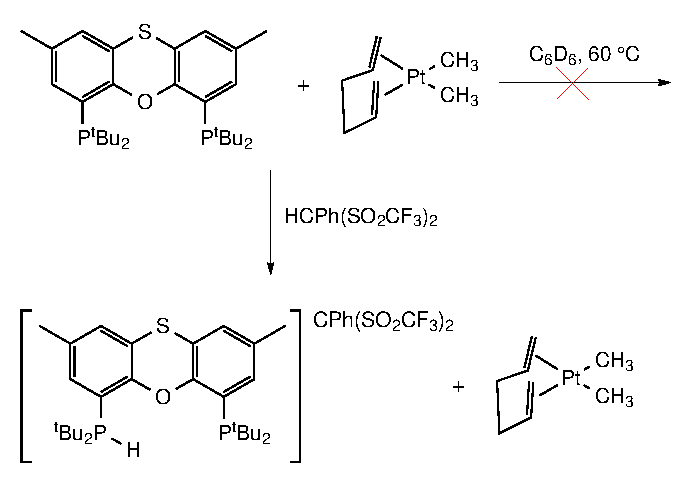
\includegraphics{../Schemes/Dimethylscheme.eps}
\caption[Attempted reaction of \ce{[Pt(hex)Me2]} and \tButhixantphos]{Attempted reaction of \ce{[Pt(hex)Me2]} and \tButhixantphos{}.  \emph{Reagents and conditions:} (i) \ce{C6D6}, 60\degC{}, (ii) \ce{HCPh(SO2CF3)2}.}
\vspace{0.2cm}
\label{scheme:PtMe2}
\end{center}
\end{scheme}
\vspace{0.2cm}

When the \tBuxantphos{} ligands were reacted with \ce{[PtCl2L2]} complexes (L = \ce{SEt2}, MeCN, \emph{t}-BuCN, \ce{L2} = 1,5-hexadiene) no \cis{} products were observed regardless of the starting material, and the reaction was fastest when the \cis{} complex \ce{[PtCl2}(\acrshort{hex})] was used due to the lability of the diene.  Due to the steric bulk of the \tBu{} substituents on the phosphorus atoms and the rigidity of the \tBuxantphos{} backbone these ligands would be expected to act as \trans{}-spanning diphosphines or tridentate \POP{} pincer ligands rather than forming \cis{} chelates.  Thus, in order for a reaction to occur between \tBuxantphos{} and [Pt(\acrshort{hex})\ce{Me2]} the system must undergo a \cis-\trans{} isomerism process.  For the dichlorides this is easily facilitated by loss of one of the chloride ligands followed by re-coordination in a \trans{} configuration.  However, methyl ligands are strong $\sigma$-donors and coordinate very strongly to Pt(II).\cite{Appleton1978}  The first step of the reaction likely proceeds with one of the phosphorus donors displacing one half of the diene (Scheme \ref{scheme:dimethyl}).   From this position the other phosphorus needs to displace the alkene forming a \cis{}-\tBuxantphos{} complex.  This could then undergo \cis-\trans{} isomerism; or the complex could isomerise first and then the phosphine could displace the alkene.  In the first case, the \cis-\tBuxantphos{} complex would be highly disfavoured due to the very large natural bite-angle of these ligands.  In either case, for the \cis-\trans{} isomerism to occur, the complex must lose a methyl ligand and these are too strongly coordinated for this to occur, especially combined with the low \trans{}-influence of the hexa-1,5-diene ligand and the moderate \trans{}-influence of the phosphorus donors.\cite{Rigamonti2010, Pregosin1980, Appleton1978}

%\tBuThixantphos was combined with \ce{[Pt(hex)Me2]} in a benzene solution.  Even with high temperatures \fixme{check what they were} and extended reaction times no reaction was observed.  An equivalent of acid was added to attempt to promote loss of methane and coordination of the diphosphine, however the acid reacted exclusively with the diphosphine instead of \ce{[Pt(hex)Me2]}.  In order to form a complex, Initial reaction between the diphosphine and \ce{[Pt(hex)Me2]} may form a complex with a dimethyl and a monodentate phosphine and hexadiene (Scheme \ref{scheme:dimethyl}).  If this forms then the steric bulk resulting from two bidentate ligands in monodentate coordination may destabilise the complex thus favouring loss of the monodentate phosphine to reform the starting materials rather than rearrangement of the strongly bound methyls into a trans configuration.

\begin{scheme}[ht]
\begin{center}
\vspace{0.5cm}
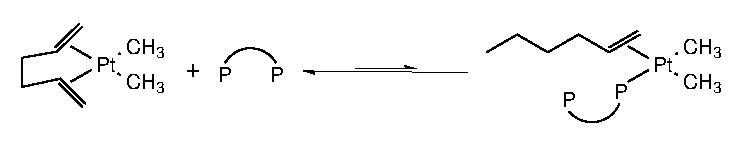
\includegraphics{../Schemes/Dimethyl.eps}
\caption[Proposed reaction between \ce{[Pt(hex)Me2]} and a diphosphine ligand]{Proposed reaction between \ce{[Pt(hex)Me2]} and a \tBuxantphos{} diphosphine ligand (PP).}
\vspace{0.2cm}
\label{scheme:dimethyl}
\end{center}
\end{scheme}
\vspace{0.2cm}

%======================================================================

\section{Reactions with \texorpdfstring{\ce{[PtCl(hex)Me]}} P}

Chloridomethylplatinum complexes are interesting due to the different properties of the chloride and methyl ligands. The methyl ligand is a much stronger $\sigma$-donor than a chloride ligand, meaning that the methyl imparts a much stronger \trans{}-influence.\cite{Appleton1978, Rigamonti2010, Pregosin1980}  The difference in the donor properties of the chloride and methyl ligands can result in asymmetric reactivity as the chloride will undergo substitution more readily than the methyl ligand.  If a \cis{}-[PtClMe(PP)] complex was formed, the two phosphorus atoms would be in different environments, which could lead to asymmetric reactions of the diphosphine.  In the more likely scenario for the \tBuxantphos{} ligand system, that \trans{}-[Pt(\tBuxantphos)ClMe] complex forms, then the strong \trans{}-influence of the methyl group may promote the dissociation of the chloride ligand

[PtCl(\acrshort{hex})Me] was chosen as the starting material due to the success of the reactions of the \tBuxantphos{} ligands with [Pt\ce{Cl2}(\acrshort{hex})].  Reaction between the \tBuxantphos{} ligands and [PtCl(\acrshort{hex})Me] was performed on an NMR-scale in \ce{C6D6} to allow the reactions to be studied as they progressed and identify any intermediates that may form.  As the reaction progressed the product precipitated out as an off-white solid.  This solid was insoluble in most common solvents except acetone-\ce{d6}.  The \tBuxantphos{} ligands and [PtCl(\acrshort{hex})Me] are insoluble in acetone, meaning that this was not suitable as the reaction solvent.  In all cases, the solution was decanted from the precipitate and the solid was dissolved in acetone-\ce{d6}, where only one species, ([Pt(\tBuxantphos)Me]Cl) was observed, indicating complete reaction (Scheme \ref{scheme:platinumchloromethyl}).    

\begin{scheme}[ht]
\begin{center}
\vspace{0.5cm}
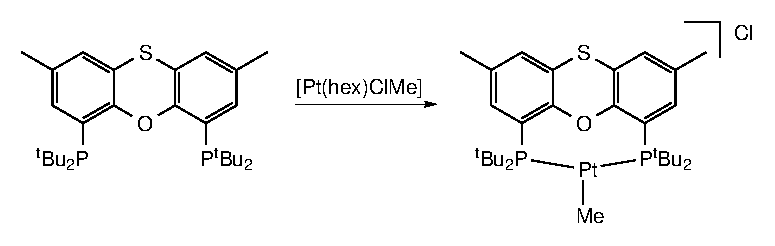
\includegraphics{../Schemes/Platinumchloromethyl.eps}
\caption[Reaction between \ce{[PtCl(hex)Me]} and \tBuxantphos{} ligands]{Reaction between \ce{[PtCl(hex)Me]} and \tBuxantphos{} ligands.  \emph{Reagents and conditions:} (i) [PtCl(hex)Me], 24 hours, room temperature (50~\degC{} \tBusixantphos{}).}
\vspace{0.2cm}
\label{scheme:platinumchloromethyl}
\end{center}
\end{scheme}
\vspace{0.2cm}

The speed of the reaction varied between the three ligands.  With \tBuxantphos{} the reaction was fastest, reaching completion in 48 hours at room temperature.  \tBuThixantphos{} reacted slightly more slowly, with completion observed after 72 hours.  \tBuSixantphos{} was the slowest of the three systems; little reaction was observed after 72 hours at room temperature, however after 24 hrs of heating at 50 \degC{} the reaction was complete by NMR spectroscopy.  This difference in reactivity is likely the result of the bite-angle of the ligand and the amount of energy required to achieve a \trans{}-geometry.  With the larger calculated bite-angle of the \tBuxantphos{} ligand the amount of energy required to achieve a pincer geometry would be lower than that for the other ligands.  Similarly \tBusixantphos{}, with the smallest of the three natural bite-angles, would require more energy in order to achieve the coordination geometry of the product.  

Selected NMR data for the three [Pt(\tBuxantphos)Me]Cl complexes is summarised in Table \ref{table:platinummethyls}.  In the \phosphorus{} NMR spectra only one signal is observed for each of the complexes, indicating identical environments for both phosphorus atoms which implies symmetrical complexes.  Given that [PtCl(\acrshort{hex})Me] is asymmetrical and a symmetrical complex is formed, this is evidence for \trans{}-coordination of the \tBuxantphos{} ligands.  The \phosphorus{} NMR signal has shifted downfield by around 40 ppm to 48.7, 50.5, or 51.0 ppm for \tBusixantphos, \tButhixantphos{} and \tBuxantphos{}, respectively.  The peak for each complex is a singlet with \JPtP{} coupling ranging from 2763 to 2793 Hz.  If the phosphorus atom was \trans{} to a chloride we would typically expect coupling constants larger than 3000 Hz, while if it was \trans{} to a methyl ligand we would expect values below 2000 Hz.  A coupling constant of around 2800 Hz is generally indicative of phosphorus \trans{} to an atom with a similar \trans-influence, in this case another phosphorus.  Furthermore this coupling is of similar magnitude to the coupling constant observed for the [Pt(\tBuxantphos)\ce{Cl2}] complexes (2686--2721 Hz).  Both of these points strongly indicate a \trans{}-coordination geometry for the complex.

\begin{sidewaystable}[htp]
\caption[Selected NMR Data for [Pt(\tBuxantphos)Me{]}Cl complexes.]{Selected NMR Data for [Pt(\tBuxantphos)Me]Cl complexes in acetone-\ce{d6}  Values for the \XJXX{}{PtX} coupling constants are given in brackets ($\Delta\delta$ = $\delta$\sub{complex} - $\delta$\sub{free ligand}).}
\vspace{1em}
\label{table:platinummethyls}
\small
\begin{center}
\begin{tabular}{l c c c c c}
	\toprule
	~ & \multicolumn{2}{c}{\bfseries{\phosphorus}} & \bfseries{\proton} & \multicolumn{2}{c}{\bfseries{\carbon}} \\
	\cmidrule(lr){2-3} \cmidrule(lr){4-4} \cmidrule(lr){5-6} 
	~\bfseries{Diphosphine} & \bfseries{$\delta/$ppm} &\bfseries{$\Delta\delta/$ppm}&\bfseries{\ce{Pt-CH3} $\delta/$ppm} & \bfseries{\ce{Pt-CH3} $\delta/$ppm} & \bfseries{$\Delta \delta$ C-O $/$ppm} \\
	\midrule		
	~\tBuSixantphos	& 48.7 (2763) & 40.3 & 2.01 (98.6) & -22.7 (780.5) & 3.0\\
	~\tBuThixantphos	& 50.5 (2793) & 41.0 & 1.94 (97.4) & -23.8 (777.2) & -1.5\\
	~\tBuXantphos{}	& 51.0 (2788) & 40.8 & 1.92 (97.4) & -23.9 (774.6) & 0.3\\
	\bottomrule{}
\end{tabular}
\end{center}
\end{sidewaystable}

The position of the \emph{O}-\emph{ipso} carbon in the \carbon{} NMR spectrum can be indicative of coordination of the oxygen to a metal centre.  In this particular case the peak for \tBusixantphos{} moves 3.0 ppm downfield from the uncoordinated ligand, while the peak for \tBuxantphos{} shifts by only 0.3 ppm downfield and the peak for \tButhixantphos{} shifts 1.5 ppm upfield comparing the free ligand with the [Pt(\tBuxantphos)Me]Cl complexes.  This is no clear indication of whether the oxygen is coordinated to the metal centre or not.  One of the reasons for this inconsistency is the insolubility of the free ligand in acetone, meaning that we are comparing the data for the free ligand in \ce{CDCl3} with the complex in acetone-\ce{d6}.  Peaks frequently shift depending on the solvent, meaning that no  conclusions can be drawn from the position of the \emph{O}-\emph{ipso} \carbon{} NMR signal in this case.  The solubility of the complex is indicative of the chloride dissociating from the metal centre.  The [Pt(\tBuxantphos)Me]Cl complexes are insoluble in the non-polar \ce{C6D6}, whereas they are very soluble in polar acetone-\ce{d6}.  This is consistent with a charged species forming in solution which could result from the loss of the chloride ligand.  Furthermore, in the [Pt(\tBuxantphos)\ce{Cl2}] complexes the chloride was observed to dissociate readily.  In this case the high \trans-influence character of the methyl ligand would promote the loss of the chloride ligand.  In addition, the strong $\sigma$-donor ability of the methyl ligand would mean that the oxygen atom would be coordinated in an extremely weak fashion and would donate less electron density when in [Pt(\tBuxantphos)Me]Cl compared with [Pt(\tBuxantphos)Cl]Cl.  

The peaks for the methyl ligand in the \proton{} and the \carbon{} NMR spectra can give additional information about the nature of the complex.  In the \proton{} NMR spectrum the peak appears between 1.92 and 2.01 ppm as a triplet with platinum satellites.  Coupling to two phosphorus atoms in the same environment generates the triplet with a three-bond \JPH{} coupling constant of 5.4--5.5 Hz, indicative of a \cis{} relationship between the phosphorus atoms and the methyl ligand, consistent with a \trans-spanning diphosphine ligand.  The value of the two-bond platinum-proton coupling constant on the methyl ligand ranges from 97.4 Hz for both \tBuxantphos{} and \tButhixantphos{}, to 98.6 Hz for \tBusixantphos.  This is a very large coupling constant for a platinum methyl ligand and is indicative of a ligand \trans{} to the methyl which has a very low \trans{}-influence.  This is also reflected in the \carbon{} NMR spectrum where the methyl ligands appear at between -22.7 and -23.9 ppm with coupling constants of 774.6--780.5 Hz.  The large upfield shift of the methyl ligand from the typical position of an organic methyl substituent (5-30 ppm\cite{Silverstein2005}) arises from the additional electron density as a result of coordination.  The chemical shift of the methyl carbon, together with the value of \JPC{} is largely the result of the ligand in the \trans{} position.  Previous work both in our group\cite{Zayya2012, Zayya2012b} and by others\cite{Scollard2001} has shown that methyl ligands \trans{} to a moderate $\sigma$ donor such as a phosphorus appear at 5--15 ppm in the \carbon{} NMR spectrum, with a platinum-carbon coupling constant of around 700 Hz.  In contrast, when the methyl is \trans{} to a weak $\sigma$-donor ligand such as a nitrogen donor the methyl shifts upfield to around -10-- -25 ppm with larger coupling constants of around 800 Hz.  In this case values of -22.7 to -23.9 for the \carbon{} chemical shift and values of \JPtC{} between 774.6--780.5 Hz clearly indicate that the methyl ligand is \trans{} to a weak $\sigma$-donor such as a chloride or an oxygen.  The value of \JPtC{} is lowest for \tBuxantphos{} and highest for \tBusixantphos{} suggesting a series of O-\trans{} influence for the three ligands of \tBusixantphos{} \textless{} \tButhixantphos{} \textless{} \tBuxantphos{}.

%Reaction with \ce{[Pt(hex)ClMe]} is much faster than either the \ce{[Pt(hex)Cl2]} or \ce{[Pt(hex)Me2]}.  This may be due to the faster reorganisation to a \emph{trans} geometry as a result of the stronger \emph{trans} influence of the methyl to promote loss of the chloride.  A single product is observed as a single sharp peak in \ce{d6-acetone} at 50.5 ppm (\JPtP{} = 2793 Hz).  This indicates \emph{trans}-coordination of the diphosphine.  Contrary to the reaction with \ce{[Pt(hex)Cl2]}, the complex that forms exclusively is a tridentate methyl complex (Scheme \ref{scheme:platinumchloromethyl}).  Due to the high \emph{trans} influence of the methyl the loss of the chloride is promoted and this is the only product even without the addition of \ce{NH4PF6} to promote the reaction.  

%The platinum methyl appears in the \proton{} NMR spectrum at 1.94 ppm as a triplet (coupling to both phosphorus atoms) with platinum satellites of 97.4 Hz.  This is very large for a two-bond platinum coupling and is indicative of a very weakly bound group \emph{trans} to the methyl.  Similar complexes reported previously include \fixme{reference ingleson2004 and others?} which have similar platinum couplings.  However the resonance for the methyl in the \carbon{} NMR spectrum is present at -23.8 ppm as a triplet with platinum satellites of 777.2 Hz.  To the best of our knowledge this is the largest reported platinum coupling constant to a methyl carbon.  All of this data supports the structure proposed as not having an interaction between the oxygen and the platinum.  Although there may be one present it is very weakly bound.  The most similar NMR data has platinum methyls \emph{trans} to weakly bound agostic interactions of isopropyl or t-butyl groups.  In these cases no evidence of the agostic interaction was seen in the NMR spectra it was only observed in the X-ray crystal structure.  Low temperature NMR down to -80~\degC{} showed no evidence for an agostic interaction.  It is also likely that as t-Bu thixantphos has an oxygen present close to the platinum that this would coordinate preferentially to forming an agostic.  

Based on the relative reactivity of the \tBuxantphos{} ligands with [PtCl(\acrshort{hex})Me] and the NMR data, [Pt(\tBuxantphos)Me]Cl is proposed as the product.  However, the coordination of the oxygen has not been established conclusively.  Two related complexes have been reported: [PdMe(\ce{P^{t}Bu3)2]+} and [PtMe(\ce{P^{i}Pr3)2]+}, the solid state structures of which have been determined by X-ray crystallography (Figure \ref{crystal:PtMe}).\cite{Ingleson2004, Walter2013}  Both complexes are stabilised in the solid-state by an agostic interaction from one of the isopropyl or \tBu{} methyl substituents, although they were synthesised in the presence of coordinating solvents.  The NMR spectra of each showed symmetrical molecules with no evidence for an agostic interaction, even down to -80\degC, indicating rapid exchange of the agostic interaction between the numerous C-H bonds available.  Low temperature \proton{} and \phosphorus{} NMR analysis of [Pt(\tBusixantphos)Me] was carried out from 20 to -80\degC.  No changes in the spectra were observed, except for a slight broadening of the signals due to precipitation.  This indicates that if an agostic-bond is present, the presence of 12 different \tBu{} \ce{CH3} groups (i.e. 36 different agostic possibilities) means there is ample opportunity for exchange, resulting in the apparent symmetry at room temperature.  

%The position of the methyl signal in the \carbon{} NMR spectrum changes depending on the bite-angle of the ligand with \tBusixantphos{}, the smallest bite-angle ligand of the three appearing most upfield and \tBuxantphos{}, with the largest bite-angle appearing most downfield (Table \ref{table:platinummethyls}).  The platinum-carbon coupling constant follows the same trend, with the smallest value corresponding to the smallest bite-angle \tBusixantphos{} and the largest value resulting from \tBuxantphos. 

%The coupling constant implies that the methyl carbon is most strongly coordinated to the metal centre in the \tBusixantphos{} complex.  The strength of metal-ligand bonds in square-planar complexes is highly dependent on the \trans{}-influence of the \trans{} ligand.  Assuming that all three complexes have the same ligand \trans{} to the methyl, the strength of the platinum-methyl interaction is thus inversely correlated with the bond strength of the ligand in the \trans{} position (and directly correlated with the length of the Pt-L bond).  As the natural bite-angle of the ligand increases we would expect the system to more readily form a \trans{} coordinating complex, as observed by the ease with which the platinum methyl complex is formed.  The bite-angle of the system will also impact the geometry of the complex that is formed.  The larger natural bite-angle \tBuxantphos{} ligand would likely form complexes with a larger bite-angle.  This has the result of bringing the oxygen closer to the metal centre and also making it geometrically easier to form an agostic complex with one of the \tBu{} substituents.  Hence the ligand coordinating \trans{} to the methyl would have the longest bond in the smallest bite-angle \tBusixantphos{} complex, thus resulting in the strongest Pt-Me bond and hence the largest platinum-carbon coupling constant, as observed spectroscopically.  

\begin{figure}[htbp]
        \centering
        \begin{subfigure}[b]{0.45\textwidth}
                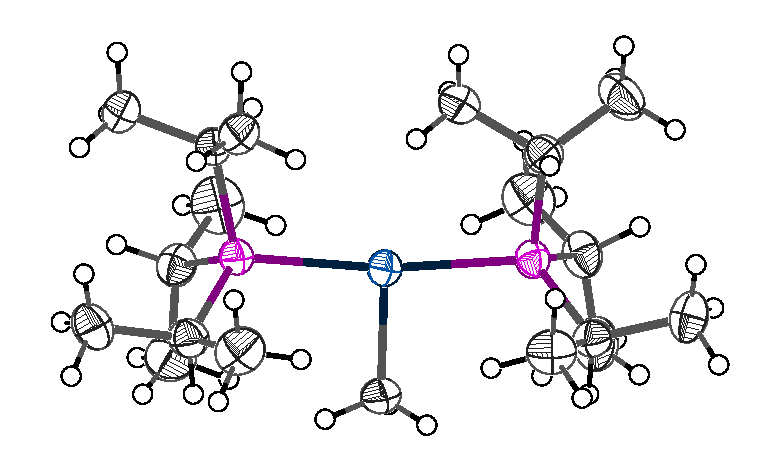
\includegraphics[width=\textwidth]{../Othercrystals/PtMe/245432.eps}
                \caption{[PtMe(\ce{P^{i}Pr3)2{]}+}}
                \label{Pt(iPr)ingleson}
        \end{subfigure}%
        ~ 
        \begin{subfigure}[b]{0.5\textwidth}
                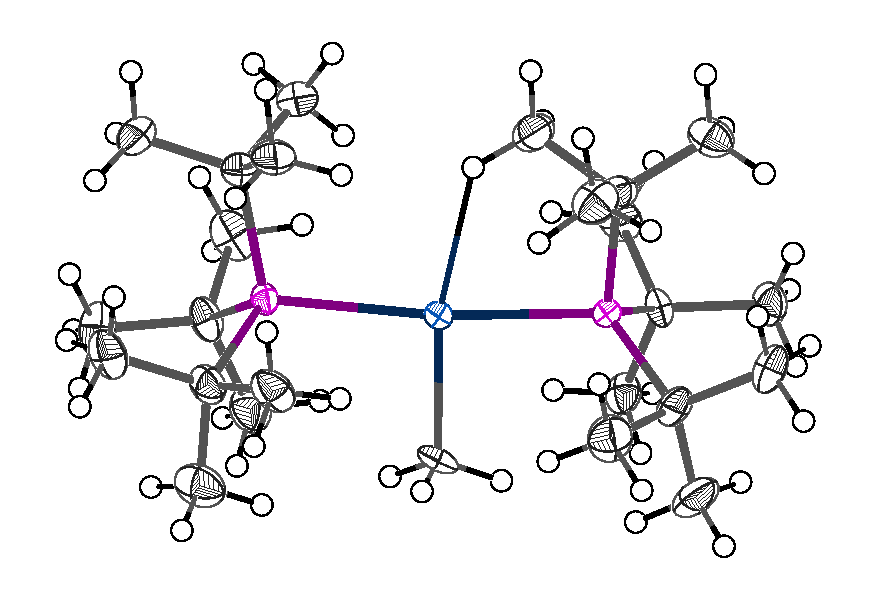
\includegraphics[width=\textwidth]{../Othercrystals/PtMe/915278.eps}
                \caption{[PdMe(\ce{P^{t}Bu3)2{]}+}}
                \label{Pt(tBu)Walter}
        \end{subfigure}
        \caption[X-ray crystal structures of [PtMe(\ce{P^{i}Pr3)2{]}+} and [PdMe(\ce{P^{t}Bu3)2{]}+}]{X-ray crystal structures of [PtMe(\ce{P^{i}Pr3)2{]}+}\cite{Ingleson2004} and [PdMe(\ce{P^{t}Bu3)2{]}+}\cite{Walter2013}.  Counterions omitted for clarity.}
        \label{crystal:PtMe}
\end{figure}

On the basis of the spectroscopic analysis and the structures of similar compounds there are three plausible structures for the product from reaction between [PtCl(\acrshort{hex})Me] and the \tBuxantphos{} ligands; all contain the \tBuxantphos{} ligand in a \trans{}-configuration and a methyl group.  The fourth coordination site on the platinum could either be occupied by a chloride ligand, an agostic interaction from one of the many \tBu{} C-H bonds, or by a very weak interaction with the oxygen in the backbone of the \tBuxantphos{} ligands.  The absence of the chloride ligand was confirmed by reaction between [Pt(\tBuxantphos)Me]Cl and \ce{NH4PF6} on an NMR-scale.  Over the course of several days no change was observed in the \proton{}, \carbon{} or \phosphorus{} NMR spectra except for the appearance of a septet in the \phosphorus{} NMR spectrum and a doublet in the \fluorine{} NMR spectrum indicative of a non-coordinating \ce{PF6-} counterion (\ce{NH4PF6} is insoluble in acetone-\ce{d6}).  As no change was observed in the NMR spectra upon cooling to -80\degC{}, the fourth coordination site could be occupied either a rapidly exchanging agostic interaction or the oxygen in the backbone (Scheme \ref{scheme:pinceragostic}).

\begin{scheme}[ht]
\begin{center}
\vspace{0.5cm}
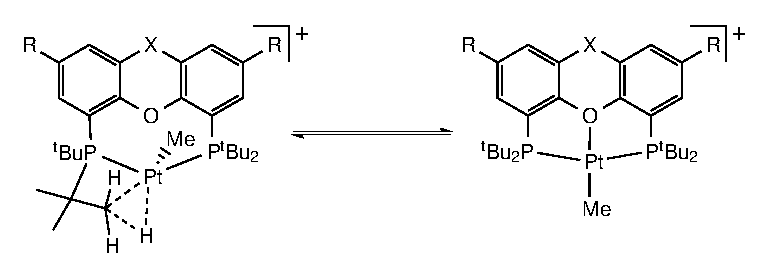
\includegraphics{../Schemes/Pinceragostic.eps}
\caption[Equilibrium between [Pt(\tBuxantphos)Me{]} and [Pt(\tBuxantphosk)Me{]}]{Equilibrium between [Pt(\tBuxantphos)Me] and [Pt(\tBuxantphosk)Me{]}.}
\vspace{0.2cm}
\label{scheme:pinceragostic}
\end{center}
\end{scheme}
\vspace{0.2cm}
\subsection{Computational Results}

Computational modelling was used to determine whether the three [Pt(\tBuxantphos)Me]X complexes  take the form of a pincer complex [Pt(\tBuxantphosk)\ce{Me]+}, or whether an agostic interaction from the \tBu{} groups is formed instead.  Structural models of both of these isomers were optimised and their vibrational frequencies were calculated using density functional theory using a B3LYP functional\cite{Becke1993, Lee1988, Vosko1980, Stephens1994} with the def2-TZVP basis set\cite{Andrae1990, Weigend2005}.  Selected bond lengths and angles are given in Table \ref{table:PtMeagostic} and \ref{table:PtMepincer} for the agostic and pincer complexes respectively.

\begin{table}[htp]
\caption[Selected bond lengths and angles for [Pt(\tBuxantphos)\ce{Me{]}+}]{Selected bond lengths and angles calculated for the agostic complexes [Pt(\tBuxantphos)\ce{Me]+}.}
\vspace{1em}
\label{table:PtMeagostic}
\small
\begin{center}
\begin{tabular}{l c c c}
	\toprule
	~\bfseries{Ligand} & \bfseries{Pt-Me $/$\si{\angstrom}} & \bfseries{Pt-H $/$\si{\angstrom}}& \bfseries{P-Pt-P $/$\degrees{}} \\
	\midrule		
	~\tBuSixantphos	& 2.051	& 2.763 	& 153.9	\\
	~\tBuThixantphos	& 2.052	& 2.828 	& 153.7 	\\
	~\tBuXantphos{}	& 2.051	& 2.868	& 153.2	\\ 
	\bottomrule{}
\end{tabular}
\end{center}
\end{table}

\begin{table}[htp]
\caption[Selected bond lengths and angles for [Pt(\tBuxantphosk)\ce{Me{]}+}]{Selected bond lengths and angles calculated for the pincer complexes [Pt(\tBuxantphosk)\ce{Me]+}.}
\vspace{1em}
\label{table:PtMepincer}
\small
\begin{center}
\begin{tabular}{l c c c}
	\toprule
	~\bfseries{Ligand} & \bfseries{Pt-Me $/$\si{\angstrom}} & \bfseries{Pt-O $/$\si{\angstrom}} & \bfseries{P-Pt-P $/$\degrees{}} \\
	\midrule		
	~\tBuSixantphos	& 2.052	& 2.323 	& 165.7 \\
	~\tBuThixantphos	& 2.053	& 2.277	& 164.4 \\
	~\tBuXantphos{}	& 2.053	& 2.256	& 164.4 \\ 
	\bottomrule{}
\end{tabular}
\end{center}
\end{table}

Little variation is present in the bond lengths and bite-angles for the three ligands in either the pincer or the agostic complex.  The platinum-methyl bond length varies by only 0.001 \si{\angstrom} between the three agostic and the three pincer complexes, and by only 0.002 \si{\angstrom} across all six of the structures.  Similarly, the bite-angles show little difference among the complexes despite the difference in the natural bite-angles for the ligands.  The platinum-oxygen bond length for the pincer complex shows a decrease with the increasing natural bite-angle of the ligand such that the \tBusixantphos{} complex has the longest Pt-O bond.  A similar trend is present for the Pt-H bond length in the agostic complexes, where the longest Pt-H distance is for the \tBusixantphos{} system and the shortest Pt-H distance is for the \tBuxantphos{} complex.  These are consistent with the observed changes in the \carbon{} NMR spectrum for the methyl ligand, whereby the \tBusixantphos{} complex has the largest value of \JPtC{} and \tBuxantphos{} has the smallest.  Decreasing the Pt-O or Pt-H bond lengths will increase the \trans{} influence of the ligand as a result of increased $\sigma$ donation from the ligand to the platinum, leading to a lower platinum-carbon coupling constant.  

The Gibbs free energy for the each of the complexes was also calculated (Table \ref{table:PtMeenergies}).  The agostic complexes were consistently higher in energy than the pincer complexes, indicating that conversion from the agostic to the pincer is an exothermic process generating 106, 111, or 122 \si{\kilo\joule\per\mole} of energy.  This suggests that the pincer complex is likely the thermodynamically favoured product in the reaction between [PtCl(\acrshort{hex})Me] and the three \tBuxantphos{} ligands (Scheme \ref{scheme:pinceragostic}).  The value for $\Delta$\emph{G} appears to be correlated with the natural bite-angle of the ligands.  This indicates that although the three diphosphine ligands produce complexes with similar bite-angles, the natural bite-angle of the ligand can impact the stability of the starting and final complexes.  

%The reaction with [PtCl(\acrshort{hex})Me] was observed to be fastest with \tBuxantphos{} and slowest with \tBusixantphos{}, while computationally we observe that \tBuxantphos{} has the most negative value for $\Delta$\emph{G} and \tBusixantphos{} has the least negative value.  

\begin{table}[htp]
\caption[Gibbs free energies calculated for agostic and pincer [Pt(\tBuxantphos)\ce{Me{]}+}]{Gibbs free energies calculated for the agostic and pincer complexes [Pt(\tBuxantphosk)\ce{Me]+}.  All values are in \si{\kilo\joule\per\mole}}
\vspace{1em}
\label{table:PtMeenergies}
\small
\begin{center}
\begin{tabular}{l c c c}
	\toprule
	~\bfseries{Ligand} & \bfseries{Agostic \emph{G}} & \bfseries{Pincer \emph{G}} & \bfseries{$\Delta$\emph{G}} \\
	\midrule		
	~\tBuSixantphos	& -6245006	& -6245113 	& -106 \\
	~\tBuThixantphos	& -6527190	& -6527301	& -111 \\
	~\tBuXantphos		& -5584828	& -5584950	& -122 \\ 
	\bottomrule{}
\end{tabular}
\end{center}
\end{table}

While the relative thermodynamic preference between the pincer and the agostic has been established, the reaction occurring is actually dissociation of a chloride from the [Pt(\tBuxantphos)ClMe] complexes forming either the pincer or the agostic complex.  The energy changes for these reactions are given in Tables \ref{table:PtClMe-Pincer} and \ref{table:PtClMe-Agostic}.  In this case we see that under standard gas-phase \gls{DFT} conditions, neither the pincer nor the agostic complex is lower in energy than the [Pt(\tBuxantphos)ClMe] starting material.  However, significantly less energy is required for the conversion to the pincer than to the agostic.  

\begin{table}[htbp]
\caption[Energy change for the conversion of the [Pt(\tBuxantphos)ClMe{]} to the pincer complex]{Energy change for the conversion of the [Pt(\tBuxantphos)ClMe{]} to the pincer complex.}
%\vspace{1em}
\label{table:PtClMe-Pincer}
	\begin{center}
	[Pt(\tBuxantphos)ClMe] $\rightarrow$ [Pt(\tBuxantphosk)Me] + \ce{Cl-}
	\small
\begin{tabular}{l c c c c c}
	\toprule
	~ & \multicolumn{5}{c}{\bfseries{$\Delta$E, \si{\kilo\joule\per\mole}}} \\
	\cmidrule(lr){2-6} 
	~\bfseries{Ligand} & \bfseries{Solvent Free} & \bfseries{\ce{(CH3)2CO}} &\bfseries{\ce{C6H6}}&\bfseries{\ce{CHCl3}} & \bfseries{\ce{CH2Cl2}} \\
	\midrule		
	~\tBusixantphos 	& 341.2	& -45.6	& 100.4 	& 11.7	& -24.7\\
	~\tButhixantphos	& 349.7	& -38.3	& 109.2	& 20.0	& -17.0\\
	~\tBuxantphos		& 337.5	& -52.7	& 97.2	& 7.4		& -30.4\\
	\bottomrule{}
\end{tabular}
\end{center}
\end{table}

\begin{table}[htbp]
\caption[Energy change for the conversion of the [Pt(\tBuxantphos)ClMe{]} to the agostic complex]{Energy change for the conversion of the [Pt(\tBuxantphos)ClMe{]} to the agostic complex [Pt(\tBuxantphos)\ce{Me{]}+}.}
%\vspace{1em}
\label{table:PtClMe-Agostic}
	\begin{center}
	[Pt(\tBuxantphos)ClMe] $\rightarrow$ [Pt(\tBuxantphos)\ce{Me{]}+ + Cl-}
	\small
%	\begin{center}
\begin{tabular}{l c c c c c}
	\toprule
	~ & \multicolumn{5}{c}{\bfseries{$\Delta$E, \si{\kilo\joule\per\mole}}} \\
	\cmidrule(lr){2-6} 
	~\bfseries{Ligand} & \bfseries{Solvent Free} & \bfseries{\ce{(CH3)2CO}} &\bfseries{\ce{C6H6}}&\bfseries{\ce{CHCl3}} & \bfseries{\ce{CH2Cl2}} \\
	\midrule		
	~\tBusixantphos 	& 454.2	& 54.9	& 210.0	& 117.0	& 78.2\\
	~\tButhixantphos	& 462.4	& 59.8	& 217.6	& 123.8	& 84.1\\
	~\tBuxantphos		& 462.7	& 60.4	& 218.9	& 124.9	& 84.8\\
	\bottomrule{}
\end{tabular}
\end{center}
\end{table}

Typical DFT computations are carried out for single molecules in the gas phase.  While this is applicable to a range of applications, when dealing with conversions between uncharged and charged molecules the solvent can have a significant impact on the thermodynamics of the reaction.  It has been observed experimentally with the platinum and palladium dichloride complexes that the solvent can also play a role in the formation of the pincer complexes.  As such, single-point energy calculations with a solvent correction were performed for the conversion of [Pt(\tBuxantphos)ClMe] into the pincer or the agostic complexes.  The energy changes are summarised in Tables \ref{table:PtClMe-Pincer} and \ref{table:PtClMe-Agostic} for the pincer and the agostic respectively.  The inclusion of any of the solvents drastically decreases the amount of energy required to form the product, thus indicating that the solvent is important for these reactions.  Under experimental conditions the reaction is performed in benzene from which the product precipitates as a white solid that is only soluble in acetone (of the solvents examined).  

The energy change for conversion of the [Pt(\tBuxantphos)ClMe] complexes into the pincer is much lower than that required to form the agostic complex, regardless of solvent.  This indicates that the pincer is thermodynamically preferred over the agostic complex.  Interestingly, for the pincer complex the reaction in benzene requires the most energy, whereas the reaction in chloroform, although still an overall positive $\Delta$E value, only requires at most 20.0 \si{\kilo\joule\per\mole}.  Based on the computational results the proposed product in the reaction between the \tBuxantphos{} ligands and [PtCl(\acrshort{hex})Me] is the pincer [Pt(\tBuxantphosk)Me]Cl complex.

The reaction of a number of xantphos ligands with [Pd(cod)ClMe] has previously been studied experimentally.\cite{Zuideveld2002}  Me-xantphos is a xantphos derivative with methyl substituents on the phosphorus atoms.  Reaction of [Pd(cod)ClMe] with Me-xantphos produces exclusively \cis{}-[PdClMe(Me-xantphos)].  All of the \Phxantphos{} ligands formed [PdClMe(\Phxantphos)] complexes that displayed \cis{}-\trans{}-isomerism at room temperature.  At low temperature both the \cis{} and \trans{} isomers were observed for \Phthixantphos{} and \Phxantphos{}, while only the \cis{} complex was observed for \Phxantphos{}.  Reaction of the [PdClMe(xantphos)] complexes with \ce{AgSO3CF3} produces the pincer complexes [PdClMe(xantphos-\POP{})][\ce{SO3CF3}] with all four ligands that were studied.  The difference in the coordination behaviour of these ligands and the \tBuxantphos{} complexes indicates that the direct formation of the [Pt(\tBuxantphos)Me]Cl complexes is most likely the result of the higher steric demands of the \tBuxantphos{} ligands compared to the \Phxantphos{} or Me-xantphos ligands.

%%======================================================================
%
%\section{Reactions of Pt(POP)Cl}
%
%Hybrid ligands are interesting due to their combination of different bonding atoms which can lead to differing activity in the \trans{} positions.\cite{Appleton1978}  If one of the ligating atoms is a weak donor group then the ligand can exhibit hemilability where the weakly bonding ligand can be displaced by something else (such as a reagent in a catalytic reaction) but the ligand still remains anchored to the metal centre and can thus still influence the reaction and can recoordinate rapidly once the reaction is complete thus stabilising the resting state for the catalyst.\cite{Jeffrey1979}
%
%The pincer complexes, [M(\tBuxantphosk)Cl]X (M = Pd, Pt) and [Pt(\tBuxantphos)Me]X discussed in this chapter have the potential for hemilability.  Oxygen donors typically coordinate very weakly to late transition metals such as palladium and platinum.  Hence the coordinating ether bridge in these complexes has the potential to be displaced by other ligands.  The coordination of the ether was explored briefly by NMR-scale reactions of [Pt(\tButhixantphos)Cl]\ce{PF6} with the weak $\sigma$-donor, acetonitrile and the strongly ligating carbon monoxide.  
%
%Addition of one equivalent of acetonitrile to a \ce{d6-acetone} solution of [Pt(\tButhixantphos)Cl]\ce{PF6} showed no reaction after 24 hours, although the presence of uncoordinated acetonitrile was observed by \proton{} NMR spectroscopy.  Further addition of an excess amount of acetonitrile, showed no evidence of any reaction.  Acetonitrile is a weak ligand and combined with the chelate effect of the pincer system and the steric bulk of the \tBu{} substituents the lack of activity is not unexpected.  
%
%Reaction of [Pt(\tButhixantphos)Cl]\ce{PF6} with the much stronger ligand carbon monoxide showed much more reactivity.  Initially a complex forms which has a \phosphorus{} NMR signal at 65.2 ppm with platinum satellites of 1889 Hz.  This indicates that the phosphorus is \trans{} to a ligand with a strongly \trans{} influence such as a carbonyl.  However, the system shows only one \phosphorus{} peak indicating that symmetry has been retained.  This complex goes on to react generating a species at 75.0 ppm (\JPtP = 2704 Hz) which is associated with a high field peak in the \proton{} NMR spectrum at -5.25 ppm which appears as a triplet (9.4 Hz) with platinum satellites (800.0 Hz).  The \phosphorus{} NMR data indicates the likely \trans{} coordination of the \tBuxantphos{} ligand system, while the \proton{} NMR spectrum has clear evidence for a platinum hydride.  
%
%Over time the species at 65.2 ppm disappears and a third species forms.  This product appears in the \phosphorus{} NMR spectrum at 57.0 ppm (\JPtP = 2557 Hz) again indicative of \trans{} coordination of the phosphorus atoms.  


%The complex \ce{[Pt{)Cl]PF6} where POP = tBu-thixantphos bonding through the two phosphines and the oxygen.  Has the potential for hemilability of the ether bridge.  This was investigated by reaction with carbon monoxide (Scheme \fixme{draw a scheme}).  The first complex is as expected where the carbon monoxide displaces the oxygen and coordinates to the platinum centre.  However, this then reacts (most likely with adventitious water) to displace the chloride and form a hydride complex.  This complex is only stable under an excess of carbon monoxide and readily loses CO and the oxygen recoordinates thus demonstrating hemilability.  Using \carbon{} enriched carbon monoxide allowed for further characterisation.  Selected NMR data for these compounds are summarised in Table \fixme{put a table here}.



%======================================================================

\section{Summary}

\tBuXantphos{} and \tButhixantphos{} were shown to react with [Pt\ce{Cl2}(\acrshort{hex})] forming exclusively \trans-[Pt(\tBuxantphos)\ce{Cl2}] complexes, unlike the \Phxantphos{} ligands which form exclusively \cis{} dichlorides.  The same reaction with \tBusixantphos{} produced the \trans{}-[Pt(\tBusixantphos)\ce{Cl2}] complex together with \tBusixantphos{}\ce{H+}, even in toluene and benzene, possibly due to reaction with the glass.  All of the dichloride complexes were dark red in colour, although most platinum dichloride complexes are pale or yellow.  This colour is possibly due to the unusual coordination geometry of the platinum, shown by X-ray crystallography of [Pt(\tButhixantphos)\ce{Cl2}].  The complex has a bite-angle of 151.722(15)\degrees{} and the sum of the angles around the platinum is 499.006\degrees{} showing significant distortion from the ideal square-planar geometry typically observed for platinum(II).  Analogous [Pd(\tBuxantphos)\ce{Cl2}] complexes were synthesised for \tBusixantphos, \tButhixantphos, and \tBuxantphos{} by reaction with [Pd(cod)\ce{Cl2}].  

The [Pt(\tBuxantphos)\ce{Cl2}] and [Pt(\tButhixantphos)\ce{Cl2}] complexes showed dissociation of a chloride ligand, forming [Pt(\tBuxantphosk)Cl]Cl in \ce{CDCl3} and \ce{CD2Cl2}.  The same behaviour was not observed for the palladium analogues.  The pincer complexes [M(\tBuxantphosk)Cl\ce{]+} could be formed for both platinum and palladium by counterion exchange with \ce{NH4PF6}.  Computational investigation into the chloride dissociation showed that although the formation of the pincer complexes is endothermic in almost all cases, the presence of any solvent more than halved the required energy  and the reactions in chloroform and dichloromethane were less endothermic than in benzene.  The reactions in acetone were close to neutral energy requirements with some exothermic results.  The palladium reactions required slightly more energy in all cases, consistent with the experimental results.  The calculations do not include entropy which is likely to be significantly in favour of the pincer complexes.    

The pincer complexes [Pt(\tBuxantphosk)Me]Cl were observed to form as the sole product from reaction of the \tBuxantphos{} ligands with [PtCl(\acrshort{hex})Me].  The NMR data was unclear regarding the coordination of the oxygen atom to the platinum and previous literature suggested that the platinum centre may be stabilised by an agostic interaction with one of the \tBu{} C-H bonds.  Computational investigation showed that for all three \tBuxantphos{} ligands the pincer complex is lower in energy suggesting that this the fourth coordination site on the platinum is occupied by the backbone oxygen.  From the values of \JPC{} for the methyl ligand the \tBusixantphos{} ligand has the weakest \trans{} influence and the \tBuxantphos{} ligand has the strongest.  This suggests that although computationally the bite-angles of the three ligands are the same, the natural bite-angle can predict the donor properties of the backbone oxygen.  

This chapter has presented a number of new platinum and palladium complexes with the \tBusixantphos{}, \tButhixantphos{}, and \tBuxantphos{}.  No \cis{} complexes were observed at any point, indicating the influence of \tBu{} groups on the coordination modes of the ligands.  The \trans{} complexes have the smallest observed bite-angles for square-planar complexes with \trans{}-spanning diphosphine ligands.  A number of \tBuxantphos{} pincer complexes were also reported, with [Pt(\tBuxantphos)Cl\ce{]+} and [Pt(\tBuxantphos)Me]Cl forming spontaneously with appropriate solvent choice. 	